\documentclass[final]{rc-book-2.14}
\usepackage[utf8]{inputenc}
\usepackage[T1]{fontenc}
\usepackage{rc-natbib-2.14}
\usepackage{rc-tabular-2.14}
\usepackage{rc-listing-2.14}
\usepackage{rotating}

\usepackage{graphicx}
\usepackage{float}
\usepackage{csquotes}
\usepackage{url}
%\usepackage{mathident}
\usepackage{empheq,amsmath}
\usepackage{pdflscape}

\usepackage{multirow, makecell,multicol}
\usepackage[cal=cm]{mathalfa}
\usepackage{lscape}
\usepackage{adjustbox}
\usepackage{array,longtable}
\usepackage{pifont}
\usepackage{psfrag}
\usepackage{tikz} 
\usepackage{calc}
\usepackage{mathrsfs}
\usepackage{amssymb}
\usepackage{amstext}
\usepackage{algorithm} 
\usepackage{algpseudocode}
\usepackage{soul}

\newcommand{\cmark}{\ding{51}}
\newcommand{\xmark}{\ding{55}}

\usepackage{arydshln}
\DeclareUnicodeCharacter{2212}{-}
\setlength\dashlinedash{0.2pt}
\setlength\dashlinegap{1.5pt}
\setlength\arrayrulewidth{0.3pt}

\usepackage{longtable}

%-------------------------------------------  
% Added by Eduardo 
\usepackage{minted}
% \usepackage{booktabs}
% ------------------------------------------


%hifen
\hyphenpenalty=2000
\tolerance=400

%orphan lines
\clubpenalty=10000
\widowpenalty=10000
\displaywidowpenalty=10000

\hyphenation{mo-ti-va-ting}
\hyphenation{des-cri-be}
\hyphenation{si-tua-tions}
\hyphenation{pro-cess-ing}
\hyphenation{se-ve-ral}
\hyphenation{UNIJUI}
\hyphenation{cha-rac-te-ris-tics}
\hyphenation{e-xe-cu-ted}
\hyphenation{fi-gu-re}
\hyphenation{know-ledge}
\hyphenation{a-ve-ra-ges}
\hyphenation{hy-po-the-sis}
\hyphenation{d-OSP}


\loadlanguages{english}
\settypewriterfont{\sffamily\smaller}

\newcolumntype{S}{>{\centering\arraybackslash}p{1.7cm}}
\newcolumntype{T}{p{6cm}}

%% Dirty-Tricks.tex

\newcolumntype{S}{>{\centering\arraybackslash}p{1.7cm}}
\newcolumntype{T}{p{6cm}}




%\includeonly{Abstract, MAIN}

\begin{document}



% deixar a sigla como uma 'inovação' no título maior. 
\title{ $d$-OSP -- Decentralized Open Science Platform}
 
\subtitle{A Decentralized Infrastructure for Transparent and Reproducible Research}

\author{Master's Candidate: \\ Eduardo Costa de Oliveira}
\institution{ \small{Regional University of Northwestern Rio Grande do Sul}}

\documenttype{Master's Dissertation}

\advisor{\hfill \linebreak \linebreak \linebreak \linebreak \normalsize{Supervisor:} \linebreak \small{Dr.~Rafael Zancan Frantz}  \linebreak\linebreak  \normalsize{Joint Supervisor:} \linebreak \small{Dr. Thiago Gomes Heck}}

\linebreak

\splash{
    \mbox{}\hfill%
    \psfigure[width=3.294192cm,height=2.913207cm]{fig/logo-unijui}%
    \hfill%
    \psfigure[width=3.294192cm,height=2.913207cm]{fig/logo-ppgmmc}%
    \hfill%
    \psfigure[width=3.294192cm,height=2.913207cm]{fig/logo-gca}%
    \hfill%
    \psfigure[width=3.294192cm,height=2.913207cm]{fig/logo-gpef}%
    \hfill\mbox{}
}

\date {\footnotesize{April, 2025}}

% Indexing page

\publisher{
    First published in April 2025 by \\
    Applied Computing Research Group - GCA \\
    Department of Exact Sciences and Engineering \\
    Rua Lulu Ilgenfritz, 480 - São Geraldo \\
    Ijuí, 98700-000, Brazil.
}

\copytext{
    Copyright \copyright\ \toroman{2012} Applied Computing Research Group \\
    \url{http://www.gca.unijui.edu.br} \\
    \email{gca@unijui.edu.br}
}

\rights{\defaultrights}

%\record {
%    D.1.2 [Automatic Programming];
%    D.1.3 [Concurrent Programming];
%    D.2.6 [Programming Environments]: Integrated environment, Programmer workbench;
%    D.2.10 [Design]: Representation;
%}

\support{
    This research is partially funded in Brazil by the Coordination for the Improvement of Higher Education Personnel (CAPES) and the National Council for Scientific and Technological Development (CNPq) through the following projects: 309425/2023-9 and 402915/2023-2.
}

% Minutes page

% \minutestext{\defaultminutestext{Mestre}{Modelagem Matemática e Computacional}} # Documented by EO
\minutestext{\defaultminutestext{Master’s Degree}{Mathematical and Computational Modeling}}


\minutesdate{\defaultminutesdate}

\boardmember{
    Dr. Rafael Zancan Frantz\\
    UNIJUÍ\\
    (Supervisor)
}

\boardmember{
    Dr. Thiago Gomes Heck\\
    UNIJUÍ\\
    (Joint Supervisor)
}

\boardmember{
    Dr. Fabio Paulo Basso\\
    UNIPAMPA
}

\boardmember{
    Dr. Sandro Sawicki \\
    UNIJUÍ
}


% Art page

% \artwork{
%     \{fig/eai-by-pedrinho.eps} \\
%     \bigbreak\bigbreak\bigbreak\bigbreak    
%     {Integração de Aplicações por Pedrinho, 7 anos de idade.} \\
% }

% Dedicatory page

\dedicatory{I dedicate this work to my beloved wife and sons, whose unwavering support, patience, and encouragement sustained me throughout this challenging and rewarding journey. Their love was a constant source of strength and inspiration.}


\makefront

%====================================================================
\chapter{Acronynms Index}
\label{app-acronym}
%====================================================================

\begin{description}
    \item[API - ] Application Program Interface
    \item[BCT -] Blockchain Technologies
    \item[BFT -] Bizantine Fault Tolerance
    \item[CODATA -] Committee on Data of the International Science
        Council
    \item [dApp -] Distributed Application
    \item[DLT -] Digital Ledger Technologies
    \item[ECDSA -] Elliptic Curve Digital Signature Algorithm
    \item[FAIR - ] Findable, Accessible, Interoperable, and Reusable
    \item[FOAF -] Friend of a Friend
    \item[ER -] Entity-Relationship
    \item[EVM -] Ethernet Virtual Machine
    \item [GRPC -] High performance Remote Procedure Call (RPC)
    \item[HTTP - ] Hyper Text Transfer Protocol
    \item[IPFS -] InterPlanetary File System
    \item [JSON -] JavaScript Object Notation
    \item[JSON-LD -] JSON Linked Data
    \item[LEARN -] Leveraging European Research Data Network
    \item[OpenAIRE -] Open Access Infrastructure for Research in Europe
    \item[P2P -] Peer to Peer
    \item[PBFT] - Practical Bizantine Fault Tolerance
    \item[PoS -] Proof of Stake
    \item[PoW -] Proof of Work
    \item[RDA -] Research Data Alliance
    \item[RDM -] Research Data Management
    \item[RSD -] Research Data Storage
    \item[RSA -] Rivest Shamir Addleman
    \item[WSV -] World State View
    \item[YAC -]  Yet Another Consensus



\end{description}


%==================================================================== 
\chapter{Acknowledgements}
\label{chp:acknowledge}
%====================================================================

\drop
I would like to acknowledge the important contributions of my advisor, Dr. Rafael Z. Frantz, whose guidance, encouragement, and steady mentorship were fundamental throughout this research. I am equally grateful to my co-advisor, Dr. Thiago Heck, for his thoughtful insights and persistent questioning, which helped sharpen the focus and depth of this work. I also extend my sincere thanks to Dr. Carlos Molina for his generous guidance and for continuously challenging my thinking in ways that significantly enriched this study.

%====================================================================
\chapter{Abstract}
\label{chp:general-abstract:english}

%====================================================================

\begin{quotation}[American Theoretical Physicist (1918 - 1988)]{Richard Feynman}
    The first principle is that you must not fool yourself \\ and you are the easiest person to fool.
\end{quotation}

\drop  The scientific community is confronted with a critical challenge: the high rate of failed research reproductions, which calls into question the validity and reliability of scientific results. Although the causes of irreproducibility are diverse, issues surrounding data access, transparency, and integrity are particularly significant. The lack of effective mechanisms to support reproducibility contributes to reduced accuracy, inflated research costs, and declining trust in scientific progress. To address this challenge, we propose a Decentralized Open Science Platform that leverages decentralized technologies such as blockchain, smart contracts, and the InterPlanetary File System to advance the adoption of Open Science principles. This study examines how these technologies can improve data sharing and support reproducibility across various scientific fields. By developing an artifact, we evaluate both the benefits and the technical hurdles of integrating these technologies, aiming to foster a more transparent, reliable, and trustworthy scientific ecosystem. The findings from this research offer insight into how decentralized infrastructures can help close reproducibility gaps and reinforce the integrity of scientific inquiry.


%====================================================================
\chapter{Resumo}
\label{chp:general-abstract:portuguese}
%====================================================================

\begin{quotation}[Físico Teórico Americano (1918 - 1988)]{Richard Feynman}
    O primeiro princípio é que você não deve enganar a si mesmo \\ e você é a pessoa mais fácil de enganar.
\end{quotation}

\drop A comunidade científica enfrenta um desafio crítico: a elevada taxa de falhas na reprodução de pesquisas, que compromete a validade e a confiabilidade dos resultados científicos. Embora as causas da irreprodutibilidade sejam diversas, questões relacionadas ao acesso, transparência e integridade dos dados desempenham um papel especialmente relevante. A ausência de mecanismos eficazes para sustentar a reprodutibilidade contribui para a redução da precisão, o aumento dos custos de pesquisa e a perda de confiança no progresso científico. Para enfrentar esse desafio, propomos uma Plataforma Descentralizada de Ciência Aberta que emprega tecnologias descentralizadas, como blockchain, contratos inteligentes e o InterPlanetary File System, com o objetivo de fortalecer a adoção dos princípios da Ciência Aberta. Este estudo investiga como essas tecnologias podem melhorar o compartilhamento de dados e apoiar a reprodutibilidade em diferentes áreas científicas. Por meio do desenvolvimento de um artefato, avaliamos tanto os benefícios quanto os desafios técnicos da integração dessas tecnologias, buscando promover um ecossistema científico mais transparente, confiável e robusto. Os resultados desta pesquisa oferecem subsídios sobre como infraestruturas descentralizadas podem contribuir para mitigar as lacunas de reprodutibilidade e reforçar a integridade da investigação científica..


%====================================================================
\chapter{Resumen}
\label{chp:general-abstract:spanish}
%====================================================================

\begin{quotation}[Físico Teórico Estadounidense (1918 - 1988)]{Richard Feynman}
    El primer principio es que no debes engañarte a ti mismo \\ y tú eres la persona más fácil de engañar.
\end{quotation}

\drop La comunidad científica se enfrenta a un desafío crítico: la alta tasa de fallos en la reproducción de investigaciones, lo que pone en duda la validez y la fiabilidad de los resultados científicos. Aunque las causas de la irreproducibilidad son diversas, los problemas relacionados con el acceso, la transparencia y la integridad de los datos desempeñan un papel especialmente importante. La falta de mecanismos eficaces para respaldar la reproducibilidad contribuye a una menor precisión, mayores costes de investigación y una pérdida de confianza en el avance científico. Para abordar este desafío, proponemos una Plataforma Descentralizada de Ciencia Abierta que emplea tecnologías descentralizadas como blockchain, contratos inteligentes y el InterPlanetary File System, con el fin de promover la adopción de los principios de la Ciencia Abierta. Este estudio examina cómo estas tecnologías pueden mejorar el intercambio de datos y fomentar la reproducibilidad en distintas disciplinas científicas. A través del desarrollo de un artefacto, evaluamos tanto los beneficios como los desafíos técnicos de integrar estas tecnologías, con el objetivo de contribuir a un ecosistema científico más transparente, fiable y sólido. Los resultados de esta investigación ofrecen perspectivas sobre cómo las infraestructuras descentralizadas pueden ayudar a cerrar las brechas de reproducibilidad y fortalecer la integridad de la investigación científica.


\mainmatter


%====================================================================
\chapter{Introduction}
\label{chp:introduction}
%====================================================================

\begin{quotation}[Roman Poet (2 AC)]{Juvenal}
    Quis custodiet ipsos custodes? \\ Who will guard the guards themselves?
\end{quotation}


\drop The purpose of this chapter is to introduce the context, motivation, and scope of the research presented in this dissertation. It outlines the reproducibility challenges faced in contemporary scientific practice and frames the relevance of decentralized technologies in addressing these issues. By situating the problem within the broader movement of Open Science, this chapter defines the research objectives and presents the foundational concepts that guide the development of the proposed solution. Provide a clear understanding of the problem domain, the research questions addressed, and the overall structure of the work.


The chapter begins by establishing the research context in Section~\ref{chp:intro:sec:context}. Section~\ref{chp:intro:sec:motivation} presents the motivation behind the study, followed by the main and specific objectives outlined in Section~\ref{chp:intro:sec:objectives}. The methodological approach adopted is described in Section~\ref{chp:intro:sec:methodology}. Section~\ref{chp:intro:sec:res_hyp} introduces the research hypothesis along with its rationale, while Section~\ref{chp:intro:sec:contributions} summarizes the key contributions. Finally, the structure of the dissertation is presented in Section~\ref{chp:intro:sec:structure}, providing an overview of the subsequent chapters.



\newpage


%-------------------------------------------------------------
\section{Research Context}
\label{chp:intro:sec:context}
%-------------------------------------------------------------


The reproducibility crisis in science arises when researchers fail to replicate the results of a study, even when using the same methods and materials. This issue is prevalent across scientific disciplines where replication is essential for validating findings, advancing knowledge, and maintaining public trust in research.

Concerns about transparency and reproducibility have intensified in recent years. Studies indicate that a significant proportion of published research does not withstand rigorous scrutiny when retested, raising doubts about the reliability of scientific knowledge. This crisis results in wasted resources, misdirected efforts, and diminished confidence in research findings. Despite various efforts to improve reproducibility and better reporting guidelines such as PRISMA (Preferred Reporting Items for Systematic reviews and Meta-Analyses) \cite{Pagen71}, ARRIVE (Animal Research Reporting of In Vivo Experiments) \cite{percie2020arrive} and FAIR (The FAIR Guiding Principles for scientific data management and stewardship) \cite{wilkinson2016fair}, significant challenges remain in ensuring that research findings are consistent, transparent, and verifiable.

Several factors contribute to this challenge, including flawed study designs, data quality issues, unreliable measurement tools, and inconsistent research practices. Poorly designed studies may overlook critical variables, while inadequate measurement tools can produce misleading results. Furthermore, incomplete reporting or the omission of key methodological details can hinder independent verification of findings \cite{freedman_economics_2015}.

A promising approach to addressing reproducibility issues lies in the adoption of Open Science \cite{foster_open_2017}, both as a movement and as a methodological framework that fosters transparency, collaboration, and accessibility in research. Open Science promotes unrestricted access to research outputs, including publications, datasets, code, methodologies, and protocols, enabling verification and reuse while reducing barriers to scientific progress. By advocating for systematic, reproducible, and accessible research practices, Open Science enhances accountability and trust within the scientific community. However, despite its transformative potential, its current implementations encounter significant technical and structural limitations, particularly in scalability, consistency, and automation. Existing infrastructures often rely on centralized repositories and fragmented systems that lack transparency, are vulnerable to manipulation or demand extensive manual oversight to ensure verifiability.

To overcome these challenges, decentralized technologies offer a robust proposition that aligns with the principles of Open Science while addressing its technical constraints. Blockchain technology ensures the immutability and integrity of research records, preventing unauthorized modifications, tampering and traceability. IPFS ( InterPlanetary File System) provides decentralized and persistent data storage, eliminating single points of failure and ensuring long-term accessibility of research outputs. Smart contracts facilitate the automated enforcement of predefined research-sharing policies reducing the need for intermediaries and fostering trust in collaborative environments. By integrating these decentralized technologies, it becomes possible to construct an infrastructure that not only upholds Open Science principles but also strengthens reproducibility by delivering secure, transparent and verifiable mechanisms for data sharing and validation across scientific disciplines.

Building upon these foundations, this dissertation proposes the development of a structured artifact designed to provide a transparent framework for documenting, validating and disseminating research outputs. This artifact will accommodate diverse materials, including reports, protocols, datasets, images and videos, ensuring secure and accessible record-keeping. By leveraging decentralized technologies, the proposed artifact targets the enhancement of methodological rigor, support independent verification of scientific findings and ultimately contribute to a more trustworthy and reproducible scientific ecosystem.

The scientific community has long recognized the importance of reproducibility in ensuring the validity and accuracy of research findings. Reproducibility refers to the ability of researchers to replicate another researcher's study or experiment, with minimal changes, to verify its results and conclusions \cite{vasilevsky_reproducibility_2013}. However, despite widespread efforts to address this issue, failed reproductions continue to be a persistent problem across various scientific domains, which not only compromises the credibility of individual studies but also undermines our collective understanding of scientific phenomena.

Studies have shown that reproducibility rates vary widely across disciplines, but even among those fields with a strong tradition of rigor, replication rates often fall short. For instance, a study published in the journal PLOS Biology found that only 22\% of papers published in top-tier journals were replicable \cite{freedman_economics_2015}. Similarly, a review of studies on reproducibility in Nature revealed that only 15\% of studies reported high levels of reproducibility \cite{landis_call_2012}.

Several interrelated factors contribute to these poor rates of reproducibility. Methodological flaws, such as sampling biases or inadequate control groups, often result in difficulties replicating findings \cite{baker2016reproducibility}. Additionally, a lack of transparency in research practices, such as insufficient reporting on methods, materials, and results, hinders independent verification and replication efforts \cite{munafo2017manifesto}. Poor data management practices further exacerbate these challenges, as issues like inadequate data documentation, lack of standardized metadata, and the absence of persistent identifiers make it difficult to retrieve, interpret, and reuse data \cite{wilkinson2016fair}. The use of proprietary or inaccessible data formats, as well as data loss due to improper storage or insufficient version control, further limits reproducibility \cite{peng2011reproducible}. Moreover, limited resources, including small research teams or restricted funding, can prevent the rigorous experimentation necessary to ensure high reproducibility levels, particularly when researchers lack access to robust data infrastructure and long-term archival solutions \cite{stark2018before}.

The need for transparency and openness in scientific research has led to the development of the Open Science movement. Open Science is a broad initiative that advocates for the transparency, accessibility and collaboration of research processes and outputs. Its tenets include making research datasets, publications, code and methodologies publicly accessible, enabling independent verification and reuse of scientific work. Open Science encourages practices such as publishing raw data, sharing code and providing comprehensive methodological descriptions that allow others to reproduce and extend findings.

Despite the substantial contributions of Open Science, the current systems and tools supporting these practices remain fragmented and often lack the scalability and consistency required for widespread adoption. As such, significant challenges in ensuring reproducibility persist, particularly when dealing with large, complex datasets, proprietary information  or sensitive research materials.

Given these challenges, the integration of decentralized technologies such as blockchain \cite{nakamoto2012bitcoin}, IPFS \cite{Benet} and smart contracts \cite{Szabo-1994}presents a potential solution to address the limitations of current Open Science frameworks. Blockchain technology offers a robust mechanism for ensuring the immutability and integrity of records, making it easier to track data provenance and verify results over time. IPFS provides a scalable, decentralized infrastructure for storing large datasets, ensuring they remain accessible and tamper-proof. Smart contracts, meanwhile, automate the verification and validation process, making it more efficient and secure. Together, these technologies enable a more transparent and accessible research ecosystem that enhances the reproducibility of scientific findings across various domains.
a.

%-------------------------------------------------------------
\section{Motivation}
\label{chp:intro:sec:motivation}
%-------------------------------------------------------------

The scientific community faces a critical challenge in ensuring the integrity and validity of research findings. Reproducibility, the ability to independently verify and replicate the results of a study, is fundamental to scientific progress. However, studies have shown that a significant proportion of published research findings cannot be reliably reproduced, with some fields reporting irreproducibility rates exceeding 50\% \cite{baker2016reproducibility}. This crisis threatens the credibility of individual researchers, academic institutions, and entire disciplines, ultimately slowing the advancement of knowledge and reducing public trust in science.

Despite ongoing efforts to improve reproducibility, the problem persists due to systemic barriers embedded within traditional research practices. Conventional publication systems prioritize novelty over transparency, funding mechanisms rarely incentivize data sharing, and peer-review processes lack the infrastructure to systematically verify research integrity. Consequently, even well-intentioned researchers struggle to ensure their work is reproducible due to inadequate tools for transparent data management, persistent identifier tracking, and independent verification.

The Open Science movement has emerged as a response to these challenges, advocating for unrestricted access to research outputs, including publications, datasets, software, and methodologies. By fostering transparency, collaboration, and standardization, Open Science aims to improve reproducibility through practices such as open data sharing, pre-registered study protocols, and transparent peer review. However, while Open Science provides a conceptual foundation for improving reproducibility, its practical implementation remains hindered by the lack of scalable, automated solutions for verifying research integrity in complex, data-intensive environments.

This dissertation proposes a decentralized solution that integrates blockchain technology, the InterPlanetary File System (IPFS), and smart contracts into scientific workflows to address reproducibility challenges within the Open Science framework. Blockchain technology ensures the immutability and verifiability of research records, preventing data manipulation and guaranteeing long-term integrity. IPFS provides a decentralized and tamper-proof storage mechanism, facilitating efficient and secure access to research outputs. Smart contracts automate validation and verification processes, reducing reliance on manual intervention and minimizing errors.

By leveraging these decentralized technologies, this research aims to establish a more transparent, secure, and reproducible scientific ecosystem. Beyond addressing current reproducibility challenges, this work seeks to strengthen the broader Open Science framework by providing tools that enable data integrity, facilitate collaboration, and support independent verification across scientific disciplines.


%-------------------------------------------------------------
\section{Objectives}
\label{chp:intro:sec:objectives}
%-------------------------------------------------------------

We present the objectives that have directed our research in the context of Open Science and the reproducibility of scientific research, which resulted in the contributions of this dissertation. This work explores the potential of distributed technologies—specifically blockchain, IPFS, and smart contracts—to improve research transparency, data integrity, and reproducibility.

\textbf{Main objective}

\begin{citeverbatim}

    Develop a platform that integrates blockchain, IPFS, and smart contracts to enhance the reproducibility, availability, and verifiability of scientific research data in alignment with Open Science principles.

\end{citeverbatim}

\textbf{Specific objectives}
\begin{itemize}
    \item Analyze the limitations of current research data management practices with respect to provenance and reproducibility;

    \item Investigate the extent to which blockchain and decentralized storage can support immutable, persistent, and verifiable research data;

    \item Design an architecture that integrates blockchain, IPFS, and smart contracts to enable transparent storage, access control, and provenance recording;

    \item Implement the proposed architecture in a functional platform that supports the secure publication and retrieval of datasets, metadata, and experiment records;

    \item Conduct experiments to evaluate the platform’s behavior in scenarios involving the registration, retrieval, and validation of experiment data, including associated metadata;

    \item Compare the reproducibility, availability, and integrity of research workflows executed with and without the use of the platform;

\end{itemize}

%-------------------------------------------------------------
\section{Methodology}
\label{chp:intro:sec:methodology}
%-------------------------------------------------------------

This study follows a structured approach grounded in the development and evaluation of a technological artifact designed to address challenges in scientific reproducibility, transparency, and data sharing. To ensure methodological rigor and practical relevance, we employ a research strategy that supports iterative refinement and empirical validation.

This research is guided by the Design Science Research (DSR) paradigm~\cite{hevner2004design}, which emphasizes the creation and assessment of artifacts as a means of generating knowledge. The objective is to design a decentralized application that facilitates scientific collaboration and improves the auditability and reproducibility of research outputs. By leveraging blockchain technology, decentralized file system, and smart contracts, the application enables researchers to securely share data, methods, and results in a transparent and verifiable manner.

The methodology consists of multiple phases. The first phase involves conceptual modeling, where the system’s architecture, data structures, and user interfaces are defined. This conceptual groundwork guides the subsequent prototyping phase, during which functional prototypes are implemented and iteratively refined based on feedback and testing.

Following prototype refinement, the final system undergoes evaluation to assess its capacity to support reproducible and transparent research practices. This includes both functional validation and alignment with Open Science principles.

The DSR methodology guiding this work incorporates three essential principles. The first is innovation, through which the research introduces a novel solution to an identified problem. The second is improvement, focusing on advancing current practices in decentralized data management. The third is validation, ensuring that the artifact undergoes  testing to demonstrate its effectiveness in meeting the research objectives.


%-------------------------------------------------------------
\section{Research Hypothesis and Rationale}
\label{chp:intro:sec:res_hyp}
%-------------------------------------------------------------


The central hypothesis of this research is that combination of these decentralized technologies: blockchain, smart contracts, and the InterPlanetary File System (IPFS), can improve reproducibility in scientific research. This hypothesis is grounded in the premise that many of the reproducibility challenges in contemporary science experiments stem from data management issues: lack of transparency in experimental protocols and study designs, restricted access to primary data, insufficient metadata, and the absence of reliable provenance tracking mechanisms.

To evaluate this hypothesis, a functional artifact will be developed and implemented, integrating blockchain, IPFS, and smart contracts within the d-OSP. The platform will support the registration, sharing, validation and provenance of research assets, such as datasets, code, and protocols and reports. The evaluation will proceed in two phases. First, a functional assessment will determine whether the system supports the reproducibility-oriented capabilities it claims to provide. Second, a scenario-based evaluation will examine how the artifact performs when used to register and verify simulated scientific workflows. These scenarios will reflect common reproducibility failure points and will be used to observe whether the system can mitigate or eliminate them.

Through this dual evaluation strategy, the research will demonstrate whether decentralized infrastructure can operationalize key principles of reproducible science, and to what extent such technologies can be practically implemented to support Open Science goals. Should the system succeed in these evaluations, the hypothesis will be considered supported.

%-------------------------------------------------------------
\section{Summary of Contributions}
\label{chp:intro:sec:contributions}
%-------------------------------------------------------------

In this section, we outline the principal contributions of this dissertation and situate them in relation to our earlier published research.

\textbf{Key Contributions of This Research}

First, we present a decentralized application that supports the transparent sharing and verification of scientific data and methods. By integrating blockchain for immutable logging, IPFS for distributed storage, and smart contracts for automated governance, we facilitate the secure and auditable dissemination of research outputs. This technological configuration strengthens reproducibility by making both data and metadata from experimental procedures verifiable and tamper-resistant.

Second, we demonstrate the artifact's value through a structured validation process. By employing iterative cycles of design, implementation, and evaluation within a DSR framework, we explore how decentralized technologies can reduce variability in research outcomes. We test the artifact through simulated use cases that highlight its capacity to mitigate reproducibility issues in data-intensive domains.

Third, we build upon our earlier research, specifically the peer-reviewed publication \textit{On the Use of Blockchain Technology to Improve the Reproducibility of Preclinical Research Experiments}~\cite{oliveira2023blockchain}, presented at the 25th International Conference on Enterprise Information Systems. That foundational work examined blockchain’s potential for improving scientific transparency. In this dissertation, we extend those insights by incorporating complementary technologies and refining their orchestration within Open Science infrastructures.

Taken together, our contributions advance the discourse on Open Science by providing a potential solution to current limitations in research data sharing. We demonstrate how decentralized architectures can uphold the principles of transparency, accountability, and accessibility offering a practical response to the ongoing reproducibility crisis in scientific research.


%-------------------------------------------------------------
\section{Dissertation Structure}
\label{chp:intro:sec:structure}
%-------------------------------------------------------------

This section provides an overview of the organization of this dissertation and the content of each chapter.

\begin{itemize}
    \item \textbf{Chapter 1: Introduction} – Establishes the overall context of the research, articulating the underlying motivation and situating the study within the broader discourse on the application of decentralized technologies and Open Science principles to enhance reproducibility. It presents the adopted methodology, introduces the research hypothesis, and provides a summary of the main contributions. The chapter concludes with an overview of the dissertation's structure.

    \item \textbf{Chapter 2: Background} – Presents the technical and conceptual foundations that support the research. It examines core concepts including decentralized and distributed systems, blockchain technologies, cryptography, smart contracts, IPFS, and the Open Science movement.

    \item \textbf{Chapter 3: Literature and Research Area Review} – Synthesizes relevant scholarly work, situating the research within ongoing debates and developments. It reviews previous initiatives that leveraged decentralized technologies to enhance reproducibility and establishes the conceptual grounding for the proposed model.
          .
    \item \textbf{Chapter 4: Proposed Decentralized Model} – Introduces the principal technical contribution of the dissertation: the d-OSP, a decentralized infrastructure represented as an artifact designed to improve reproducibility in scientific research. It outlines the platform’s architecture, data model, implementation details, and the rationale behind key design decisions. The chapter also presents an empirical evaluation of the platform’s performance and functionality.

    \item \textbf{Chapter 5: Conclusions} – Summarizes the key findings of the research and reflects on their broader implications. It revisits the hypotheses in light of the presented evidence and discusses potential avenues for future research.

    \item \textbf{Appendices and References} – The appendices include supplementary materials such as implementation details, code excerpts, and technical documentation that complement the main chapters. The references section compiles all cited scholarly sources, upholding the standards of academic transparency and rigor.

\end{itemize}

%====================================================================
\chapter{Background}
\label{chp:background}
%====================================================================

\begin{quotation}[]{Roman Poet Juvenal  2 AC}
    Quis custodiet ipsos custodes?  Who will guard the guards themselves?
\end{quotation}

\drop To support the development of the proposed Decentralized Open Science Platform, this chapter presents the technical and conceptual foundations underpinning the research.
Section~\ref{chp:background:sec:dec_dist} examines decentralized and distributed systems, Section~\ref{chp:background:sec:bct} introduces the main concepts of blockchain technologies, and Section~\ref{chp:background:sec:smart_cont} defines and contextualizes smart contracts. The InterPlanetary File System is discussed in Section~\ref{chp:background:sec:ipfs}, while the synergies between blockchain and IPFS are explored in Section~\ref{chp:background:sec:ipfs_bct_comp}. Lastly, the Open Science movement is examined in Section~\ref{chp:background:sec:os_rep}. Together, these elements form the foundational framework upon which the platform’s architecture and governance mechanisms are built.


\newpage

%====================================================================
\section{Decentralization and Distributed Systems}
\label{chp:background:sec:dec_dist}
%====================================================================

Decentralization and distributed systems are fundamental paradigms that redefine how data is processed, stored, and verified across various domains. Unlike traditional architectures that rely on a centralized entity to manage operations, decentralized systems distribute control among multiple participants \cite{coulouris2011distributed}. This approach enhances fault tolerance, ensures system resilience, and mitigates risks associated with single points of failure. Distributed systems, in turn, rely on a network of interconnected nodes to collectively maintain and process data, enabling scalability and redundancy   \cite{lamport_1978, coulouris2011distributed}. These principles underpin various modern technologies, including blockchain \cite{nakamoto2008bitcoin} and decentralized file storage networks \cite{benet2014ipfs}, which eliminate reliance on centralized intermediaries and foster transparency and security.

\subsection{The Building Blocks for Decentralization}

Blockchain technology embodies decentralization by ensuring that no single entity controls data integrity and transaction validation. Transactions are recorded in a distributed ledger that is collectively maintained by network participants through consensus mechanisms \cite{nakamoto2008bitcoin}. Using cryptographic techniques \cite{katz2020introduction} and game-theoretic incentives \cite{roughgarden2016twentyone}, the blockchain achieves trustless verification, preventing unauthorized modifications while ensuring transparency.

Similarly, the InterPlanetary File System (IPFS) uses distributed system principles to provide decentralized data storage \cite{benet2014ipfs}. Unlike conventional file storage, which relies on centralized servers, IPFS distributes files across a peer-to-peer network, addressing them based on their content rather than location. This approach not only ensures data persistence but also enhances accessibility by allowing multiple nodes to host and retrieve the same content. In contrast to blockchain, which primarily records transactions and state changes, IPFS enables efficient and scalable storage of large data objects, complementing blockchain’s immutability with a robust storage layer.

Both blockchain and IPFS exemplify the synergy between decentralization and distributed computing. Blockchain secures and verifies data integrity, while IPFS ensures scalable, redundant storage, collectively forming the foundation for decentralized applications, provenance tracking, and secure data sharing.

\subsection{Decentralized Data Management}

Blockchain technology and the InterPlanetary File System (IPFS) represent complementary solutions in decentralized systems. Blockchain serves as a distributed ledger that ensures immutability, transparency, and security through cryptographic hashing and consensus mechanisms, excelling at maintaining an auditable record of transactions and verifying data integrity \cite{nakamoto2008bitcoin}. In contrast, IPFS is a peer-to-peer distributed file system that addresses data storage challenges by organizing and retrieving content based on its hash rather than its location, enhancing resilience and efficiency by enabling distributed data hosting across a network of nodes \cite{benet2014ipfs}.

%====================================================================
\section{Blockchain}
\label{chp:background:sec:bct}
%====================================================================

Blockchain is a decentralized, immutable ledger technology designed to facilitate secure and transparent transactions within distributed networks. Initially conceptualized for the Bitcoin blockchain \cite{nakamoto2008bitcoin}, this technology has since evolved into a multi-purpose infrastructure featuring use cases in various domains, including finance, supply chain management, and digital identity verification.

The fundamental characteristics of blockchain, including decentralization, immutability, transparency, and security, make it a powerful tool for enhancing scientific reproducibility. By providing an auditable and tamper-proof record of research data and workflows, blockchain ensures data integrity and long-term verifiability. Its foundation in cryptographic principles and distributed systems enables it to support a robust infrastructure that enhances the reliability and transparency of scientific research.

\subsection{Merkle Trees}

The development of blockchain, however, did not occur in isolation. The concept of a cryptographically secured chain of blocks predates Bitcoin and draws from earlier research on distributed consensus and cryptographic techniques. A key component in blockchain structures is the Merkle tree, a concept introduced by Ralph Merkle in the 1980s \cite{goos_digital_1988}. These trees enable efficient data integrity verification by organizing hashes in a hierarchical structure, which is crucial for maintaining the integrity of blockchain data.

\subsection{Secure Time Stamping}

Building on these foundational cryptographic concepts, Stuart Haber and W. Scott Stornetta proposed a method for securely time-stamping digital documents in 1991 \cite{haber_how_1991}. This innovation was significant because it prevented backdating and tampering, laying the groundwork for immutable records. In 1992, Haber, Stornetta, and Bayer further refined this approach by incorporating Merkle trees into their time-stamping system, thereby improving efficiency and strengthening security \cite{bayer1993improving}. These advancements not only contributed to the development of blockchain but also highlighted the potential of decentralized, immutable ledgers for maintaining verifiable records.

\subsection{Public, Private and Hybrid Blockchains}

Blockchains can be categorized based on their access control and governance mechanisms into public, private, and hybrid models. Each type offers distinct advantages and trade-offs in terms of decentralization, security, scalability, and transparency.

\begin{itemize}

    \item \textbf{Public Blockchains:} Allow unrestricted participation, enabling any user to join the network, validate transactions, and maintain a copy of the ledger. These blockchains emphasize decentralization and security, ensuring data integrity through cryptographic hashing and consensus mechanisms such as Proof of Work (PoW) and Proof of Stake (PoS) \cite{nakamoto2008bitcoin}. Prominent examples include \textit{Bitcoin} and \textit{Ethereum}, which are designed to function in open, trustless environments. A defining feature of public blockchains is their transparency, as all transactions are recorded on a publicly accessible ledger. This openness makes them well-suited for scenarios requiring verifiability and censorship resistance, though it typically incurs trade-offs in scalability and performance, as each node must process and store all transactions.

    \item \textbf{Private or Permissioned Blockchains:} Restrict participation to authorized entities, making them particularly suitable for enterprise and institutional applications. Frameworks such as Hyperledger Fabric and Hyperledger Iroha are designed for regulated environments where identity verification, compliance, and access control are critical considerations \cite{cachin2016architecture}. Since private blockchains operate under a governing authority that controls access and consensus rules, they offer enhanced scalability and efficiency compared to public blockchains. Unlike PoW-based systems, permissioned blockchains often employ consensus mechanisms such as Practical Byzantine Fault Tolerance (PBFT) and Raft, which reduce computational overhead and transaction latency \cite{vukolic2017}. However, the trade-off is a reduction in decentralization, as control is concentrated within a predefined group of participants.

    \item \textbf{Hybrid Blockchains:} Integrate elements of both public and private blockchains, enabling organizations to leverage the benefits of decentralization while maintaining privacy for sensitive data. These architectures allow entities to manage a private ledger while selectively interacting with public networks for verification, auditability, or interoperability. Hybrid approaches are particularly valuable in sectors where confidentiality and transparency must coexist, such as supply chain management, financial services, and healthcare \cite{ahmed20222}. By connecting permissioned chains to public networks, hybrid models offer a balance between data privacy, operational efficiency, and the advantages of immutable public verification.

\end{itemize}

\subsection{Mining and Block Validation}

Mining is the process by which transactions are validated and added to a blockchain. In PoW-based systems, miners compete to solve cryptographic puzzles, while in PoS-based systems, validators are selected to propose and confirm blocks based on their stakes. Mining serves two key purposes: securing the network by making attacks computationally expensive and issuing new tokens as rewards. This incentive structure aligns participant behavior with the network’s security goals \cite{bonneau2015sok}. For example, Bitcoin employs PoW mining, while Ethereum 2.0 uses PoS validation.

\subsection{Consensus Mechanisms}

Consensus mechanisms are fundamental to blockchain networks, ensuring agreement among distributed nodes without requiring centralized authority. These mechanisms validate transactions and maintain the integrity of the ledger, preventing issues such as double-spending and malicious attacks.

\begin{itemize}

    \item \textbf{Proof of Work (PoW):} Requires participants, known as miners, to solve computationally intensive cryptographic puzzles. The first miner to solve the puzzle earns the right to append a new block to the blockchain and receives a block reward. This mechanism ensures network security by making it economically and computationally infeasible to manipulate the ledger. However, its reliance on high energy consumption has raised sustainability concerns \cite{narayanan2016bitcoin, sedlmeir_energy_2020}. A difficulty adjustment algorithm modulates puzzle complexity to maintain a consistent block production rate in response to changes in total network computational power.

    \item \textbf{Proof of Stake (PoS):} Offers an energy-efficient alternative to PoW by replacing mining with a staking-based validation process. In PoS systems, participants—referred to as validators—are selected to propose and attest to new blocks based on the amount of cryptocurrency they lock as collateral. This design reduces energy consumption while preserving network security and decentralization. Rather than expending computational effort, validators are incentivized to behave honestly through economic rewards and penalties. Contemporary PoS protocols often include enhancements such as dynamic staking models and slashing mechanisms, which penalize malicious behavior and reinforce protocol robustness \cite{kiayias2017}.

\end{itemize}


\subsection{Byzantine Fault Tolerance}

Byzantine Fault Tolerance (BFT) refers to the ability of a distributed system to function correctly even when some nodes fail or behave maliciously \cite{lamport1982byzantine}. Classical BFT algorithms, such as Practical Byzantine Fault Tolerance (PBFT) \cite{castro1999practical}, require \(2f+1\) honest nodes out of \(3f+1\) total nodes to tolerate up to \(f\) Byzantine faults. While PBFT offers strong consistency and finality, it assumes a fixed set of validators, making it particularly suitable for permissioned blockchain environments.

In this work, we focus on the BFT-based consensus mechanism employed by Hyperledger Iroha: Yet Another Consensus (YAC).

\textbf{YAC}

Yet Another Consensus (YAC) is a lightweight BFT algorithm tailored for permissioned blockchain networks, where validators are pre-approved entities \cite{muratov_yac_2018}. YAC emphasizes efficient communication and low-latency block validation, making it well-suited for enterprise-grade applications that demand both performance and reliability.


\textbf{Consensus Algorithm for YAC}

The YAC (Yet Another Consensus) algorithm ensures Byzantine Fault Tolerance (BFT) through a voting-based process, as follows:

\textbf{Fault Tolerance}

The network must satisfy:
\[
    n \geq 3f + 1
\]
Where:
\begin{itemize}
    \item \( n \): Total number of nodes in the network.
    \item \( f \): Maximum number of Byzantine (malicious or faulty) nodes tolerated.
\end{itemize}

This ensures that the network can tolerate up to \( f \) Byzantine nodes while still achieving consensus.

\textbf{Supermajority Agreement}
For a block to be finalized, a supermajority of nodes must agree on its hash:
\[
    v > \frac{2n}{3}
\]
Where:
\begin{itemize}
    \item \( v \): Number of votes for the block hash.
    \item \( n \): Total number of nodes.
\end{itemize}

This condition guarantees both safety and liveness in consensus.

\textbf{Voting Process}

The voting process involves two phases:
\begin{enumerate}
    \item {Proposal Phase}: A leader node proposes a block hash.
    \item {Voting Phase}: Nodes vote on the proposed hash, and votes are collected until the supermajority condition is met.
\end{enumerate}

\textbf{Finality}
Once a block achieves supermajority agreement, it is considered finalized and added to the blockchain. This ensures that all honest nodes accept the same block, preventing forks.

Consensus mechanisms, mining, and fault tolerance strategies are critical in ensuring blockchain security and functionality. The choice between PoW, PoS, and BFT-based approaches impacts the efficiency, decentralization, and security of blockchain networks. Furthermore, the distinction between public, private, and hybrid blockchains influences their applications, with public blockchains prioritizing trustlessness and private blockchains emphasizing control and efficiency. Understanding these foundational aspects enables the development of blockchain-based solutions tailored to the needs of Open Science and research reproducibility.

Hyperledger Iroha integrates YAC to ensure secure and robust consensus through a voting-based mechanism. This approach enables fault tolerance and streamlined consensus, aligning with the system's goals of scalability and operational efficiency.


\subsection{Cryptography in Blockchain}

Public key cryptography plays a fundamental role in securing blockchain networks by enabling secure transactions, identity verification, and data integrity without requiring a centralized authority \cite{narayanan2016bitcoin}. It forms the foundation for digital signatures, key management, and encryption mechanisms that ensure trust and security in decentralized environments.

\textbf{The Role of Public Key Cryptography in Blockchain}

Blockchain networks rely on asymmetric cryptography, also known as public key cryptography, to authenticate and authorize transactions \cite{rivest1978method}. Each participant holds a pair of cryptographic keys: a public key, which functions as an address to receive transactions, and a private key, which is used to sign transactions and assert ownership. When a user initiates a transaction, they produce a digital signature using their private key. This signature enables other participants to verify the transaction’s authenticity without exposing the private key itself \cite{menezes1996handbook}.

This mechanism ensures that only the rightful owner of an asset can authorize its transfer, preventing fraud and unauthorized access \cite{wood2014ethereum}. Additionally, cryptographic hashing techniques complement public key cryptography by ensuring data integrity and linking transactions in an immutable ledger \cite{merkle1988digital}.

\textbf{Commonly Used Cryptographic Ciphers and Standards}

Several cryptographic ciphers and standards are widely used in blockchain implementations to provide strong security guarantees:

\begin{itemize}
    \item \textbf{RSA (Rivest-Shamir-Adleman):} A traditional public key cryptosystem based on the difficulty of factoring large prime numbers \cite{rivest1978method}. While RSA is widely used in general cryptographic applications, its key sizes are relatively large compared to modern alternatives, making it less practical for blockchain applications.
    \item \textbf{Elliptic Curve Cryptography (ECC):} A more efficient asymmetric cryptography scheme that provides the same level of security as RSA but with significantly smaller key sizes \cite{miller1986use}. This efficiency makes ECC the preferred choice for blockchain applications.
    \item \textbf{ECDSA (Elliptic Curve Digital Signature Algorithm):} A widely adopted digital signature scheme based on ECC, used in Bitcoin and Ethereum to secure transactions \cite{johnson2001elliptic}.
    \item \textbf{EdDSA (Edwards-curve Digital Signature Algorithm):} A modern alternative to ECDSA, known for its faster signature verification and improved security properties \cite{bernstein2012high}. It is used in newer blockchain protocols like Monero.
    \item \textbf{X25519:} A secure key exchange protocol based on Curve25519, commonly used in cryptographic operations for secure communication in blockchain applications \cite{langley2016curve25519}.
    \item \textbf{Ed25519 with SHA-3:} Hyperledger Iroha natively employs Ed25519, a variant of EdDSA, combined with SHA-3 for enhanced security. This cryptographic combination ensures efficient key pair generation, digital signatures, and verification processes tailored to Iroha’s permissioned blockchain environment \cite{hyperledger_iroha}.
\end{itemize}

\textbf{Elliptic Curve Cryptography (ECC) in Blockchain}

Elliptic Curve Cryptography (ECC) is a type of public key cryptography that leverages the mathematical properties of elliptic curves over finite fields to provide strong security with smaller key sizes \cite{koblitz1987elliptic}. The security of ECC is based on the Elliptic Curve Discrete Logarithm Problem (ECDLP), which is computationally hard to solve \cite{hankerson2006guide}.

In blockchain systems, ECC is primarily used for:

\begin{itemize}
    \item \textbf{Digital Signatures:} ECC enables the creation of compact and secure digital signatures, such as those used in Bitcoin (ECDSA) and newer blockchain protocols (EdDSA and Ed25519) \cite{johnson2001elliptic, bernstein2012high}.
    \item \textbf{Key Pair Generation:} Blockchain wallets generate private-public key pairs using elliptic curves, ensuring that users can securely sign and verify transactions \cite{wu2018blockchain}. For example, Hyperledger Iroha specifically utilizes Ed25519 with SHA-3 for key pair generation, providing robust security and efficiency \cite{hyperledger_iroha}.
    \item \textbf{Scalability and Efficiency:} Due to its small key size and lower computational requirements, ECC allows blockchain networks to process transactions more efficiently while maintaining security \cite{fan2018analysis}.
\end{itemize}

Bitcoin, for instance, uses the secp256k1 elliptic curve for key generation and signing, which provides a 256-bit key length offering high security with lower processing overhead compared to traditional cryptographic methods \cite{brown2010standards}. In contrast, Hyperledger Iroha leverages Ed25519 with SHA-3 to ensure a balance between performance, security, and compatibility with modern cryptographic best practices \cite{hyperledger_iroha}.

Public key cryptography is a cornerstone of blockchain security, enabling authentication, digital signatures, and secure communication. The adoption of ECC and its derivatives, such as ECDSA and EdDSA, has significantly improved the efficiency and scalability of blockchain networks, making them resilient to attacks while minimizing computational and storage costs. Future blockchain advancements may incorporate more advanced cryptographic techniques, including post-quantum cryptography, to further enhance security in decentralized systems.


%====================================================================
\section{Smart Contracts}
\label{chp:background:sec:smart_cont}
%====================================================================

Smart contracts represent a fundamental technological innovation that automates and enforces agreements between parties without the need for trusted intermediaries. First conceptualized by Nick Szabo in the late 1990s, they were envisioned as self-executing contractual arrangements in which terms are translated into code and enforced automatically by the system itself\cite{szabo1996smart}. Szabo illustrated this concept using the analogy of a vending machine, where the mechanism guarantees the delivery of goods upon receiving correct payment, thereby minimizing the necessity for trust between parties\cite{szabo1997formalizing}.

\subsection{Operations}

From a technical standpoint, smart contracts are executable programs that encapsulate business logic and operate within virtual machines embedded in blockchain or distributed ledger infrastructures. Their implementation typically follows a structured workflow: stakeholders define functional and operational requirements; conditional logic—such as payment authorization or delivery confirmation—is formalized; developers translate this logic into code using domain-specific languages or frameworks; and the resulting contract undergoes rigorous testing and auditing prior to deployment. Once active, the contract listens for event data from trusted external inputs known as oracles. Upon detecting fulfillment of predefined criteria, the contract autonomously triggers execution\cite{simplilearn2022smart}.

This automation not only removes the need for intermediaries but also introduces transparency, auditability, and deterministic behavior in transaction processing. Every execution is permanently recorded on the blockchain, establishing an immutable trail that reinforces accountability.

\subsection{Decentralized Applications}

Within the decentralized application (dApp) ecosystem, smart contracts function as core computational units, encoding autonomous logic that operates without centralized oversight. This architecture facilitates trustless interactions among participants, allowing for complex operations such as asset transfers, service exchanges, or collaborative workflows, all without requiring mutual trust. Governance mechanisms embedded in these contracts ensure that operational rules are transparent and verifiable to all network participants. Moreover, their capacity to execute multi-party agreements algorithmically supports decentralized decision-making structures and streamlines value exchange across distributed systems\cite{alharby2017blockchain}.

\subsection{Smart Contracts for Reproducibility}

The application of smart contracts in scientific research introduces an innovative mechanism for addressing reproducibility challenges. By encoding experimental protocols, data acquisition processes, and analytical workflows into smart contracts, researchers can formalize and preserve their methodologies in a tamper-evident manner\cite{pilehchiha2022improving}. These contracts can autonomously coordinate tasks such as:

\begin{itemize}
    \item Tracking data provenance.
    \item Recording experimental parameters.
    \item Executing statistical analyses.
    \item Publishing results with cryptographic verification.
\end{itemize}

This procedural formalization ensures that research outputs are not only transparent but also replicable by other investigators, thus aligning with the broader objectives of Open Science.

Smart contracts extend the capabilities of distributed ledger technologies by introducing programmable, self-executing logic into transactional workflows. Their role in enabling decentralized governance, automating complex processes, and preserving procedural integrity positions them as a foundational element in next-generation digital infrastructures. In the context of scientific research, smart contracts can transform how reproducibility is achieved—shifting it from a manual, error-prone process to one grounded in automation, transparency, and verifiability. As the ecosystem matures, continued research is essential to address technical, ethical, and interoperability challenges, thereby unlocking their full potential across domains.

\subsection{Hyperledger Implementations}

The Hyperledger ecosystem is an open-source collaborative effort hosted by the Linux Foundation Decentralized Trust, designed to advance cross-industry blockchain technologies. Rather than a single blockchain platform, Hyperledger serves as an umbrella project encompassing a suite of modular frameworks, tools, and libraries intended for developing enterprise-grade, permissioned distributed ledger solutions. It brings together a diverse community of developers, enterprises, and academic institutions to foster innovation in areas such as supply chain, finance, healthcare, and, increasingly, scientific research. By offering a range of specialized blockchain framework, each optimized for different technical and organizational needs, Hyperledger supports the creation of scalable, secure, and interoperable distributed systems.

The Hyperledger ecosystem comprises several smart contract frameworks, each with its own architecture and set of capabilities.

\begin{itemize}

    \item \textbf{Hyperledger Fabric:} Hyperledger Fabric has progressively incorporated support for Ethereum Virtual Machine (EVM) bytecode, permitting the development of smart contracts in languages such as Solidity and Vyper. Introduced in version 1.3, this functionality facilitates the migration and creation of decentralized applications within permissioned networks, thereby broadening Fabric's applicability\cite{hyperledger2018fabric}.

    \item \textbf{Hyperledger Burrow:} Hyperledger Burrow is an Ethereum-compatible, permissioned blockchain designed to execute smart contract code on a dedicated virtual machine. Powered by the Tendermint consensus engine, Burrow achieves transaction finality and high throughput suited to proof-of-stake environments. Its role within the Hyperledger suite includes a connection to the Tendermint/Cosmos ecosystem, an Ethereum side-chain compatible with expressive smart contract languages, and a modular, customizable EVM/Solidity execution library\cite{hyperledger2019burrow}. As a complete blockchain platform, Burrow integrates a Unix-style permissioning scheme within its EVM, supporting fine-grained control over actions such as token transfers, contract deployment, and validator participation\cite{monax2020burrow}.

    \item \textbf{Hyperledger Iroha:} Hyperledger Iroha adopts a unique strategy for implementing smart contracts. While version 1 offered a constrained command set without Turing completeness, version 2 introduces Iroha Special Instructions (ISI), which enable Turing-complete computation while preserving simplicity for routine operations. Contrary to Ethereum’s model of deploying and interacting with contract instances, Iroha is structured around a core model of domains, accounts, and assets. These entities evolve through defined interactions. ISI behaves more like database triggers than autonomous smart contracts, activating in response to transactions that satisfy specific conditions\cite{hyperledger2020iroha}.

\end{itemize}

%====================================================================
\section{The InterPlanetary File System}
\label{chp:background:sec:ipfs}
%====================================================================


The InterPlanetary File System (IPFS) is a decentralized, peer-to-peer distributed file system designed to interconnect computing devices through a unified storage network \cite{benet2014ipfs}. By employing content-addressable storage and cryptographic hashing, IPFS enables the efficient sharing and retrieval of immutable data objects. Conceptually, it operates as a single, large-scale BitTorrent swarm exchanging objects within a Git-like repository. The system leverages a high-throughput, content-addressed block storage model with content-addressed hyperlinks, forming a generalized Merkle Directed Acyclic Graph (DAG). This architecture underpins various functionalities, including versioned file systems, blockchain data structures, and a more persistent and decentralized web. By integrating a Distributed Hash Table (DHT), an incentivized block exchange protocol, and a self-certifying namespace, IPFS eliminates single points of failure and minimizes the necessity for inter-node trust.

\subsection{Background and Architectural Principles}

IPFS is inspired by and synthesizes multiple established peer-to-peer technologies, including DHTs, BitTorrent, Git, and Self-Certifying Filesystems (SFS) \cite{benet2014ipfs}. While traditional web protocols such as HTTP provide an efficient means of requesting and transmitting data, they do not inherently incorporate modern file distribution strategies, resulting in limitations concerning redundancy, security, and scalability. By contrast, IPFS addresses these challenges by integrating and refining established distributed system techniques into a unified framework, ensuring efficient content retrieval and data persistence across geographically distributed nodes.

\subsection{Key Architectural Components}

IPFS is structured as a modular protocol stack, with distinct subsystems contributing to its overall functionality \cite{benet2014ipfs}:

\begin{itemize}
    \item \textbf{Identities:} Manages node identity generation and verification, typically employing static cryptographic puzzles derived from S/Kademlia.
    \item \textbf{Network:} Governs peer-to-peer communication through various transport mechanisms, including WebRTC DataChannels and uTP.
    \item \textbf{Routing:} Facilitates object discovery and peer lookup through a DHT, defaulting to a structure based on S/Kademlia and Coral.
    \item \textbf{Exchange:} Utilizes BitSwap, a block exchange protocol that promotes efficient data replication through an incentive-driven market mechanism.
    \item \textbf{Objects:} Implements a Merkle DAG to store immutable, content-addressed objects, forming the foundation for versioned data structures.
    \item \textbf{Files:} Introduces a versioned file system hierarchy inspired by Git, supporting efficient data storage and retrieval.
    \item \textbf{Naming:} Incorporates a self-certifying mutable name system, enabling dynamic reference updates for evolving datasets.
\end{itemize}

These components collectively ensure a robust and scalable approach to distributed data management, making IPFS a compelling alternative to centralized storage solutions.

\subsection{Content Addressing and Data Integrity}

A fundamental principle of IPFS is its reliance on content addressing, wherein data objects are identified by the cryptographic hash of their contents \cite{benet2014ipfs}. This methodology not only facilitates efficient deduplication but also guarantees data integrity, as any modification to an object results in a new, distinct hash. The Merkle DAG structure further enhances the efficiency of storage and retrieval processes, allowing for seamless handling of large datasets and enabling robust versioning capabilities. By leveraging cryptographic hashing, IPFS inherently verifies data authenticity and prevents unauthorized modifications.

\subsection{Routing and Peer Discovery}

IPFS employs a DHT-based routing mechanism to locate peers and retrieve specific data objects \cite{benet2014ipfs}. This approach enables highly scalable and decentralized object discovery, as network participants contribute to maintaining a distributed index of content addresses. Small data values (typically under 1KB) can be stored directly within the DHT, whereas larger datasets are distributed across multiple nodes, optimizing both redundancy and retrieval speed.

\subsection{Block Exchange and Incentive Mechanisms}

The BitSwap protocol governs IPFS’s block exchange mechanism, ensuring efficient data distribution and replication \cite{benet2014ipfs}. BitSwap operates as a marketplace where nodes trade blocks with one another, prioritizing the replication of rarer blocks to optimize availability. This economic model incentivizes participation and data persistence, ensuring that frequently accessed content remains accessible without relying on a centralized infrastructure.

\subsection{Security and Node Authentication}

Security within IPFS is underpinned by a cryptographic identity system, where nodes are identified by the hash of their public key \cite{benet2014ipfs}. This ensures that nodes can authenticate one another upon connection, exchanging public keys to verify identities. Additionally, IPFS adopts a flexible multihash format for cryptographic digests, allowing for algorithmic adaptability as cryptographic standards evolve.

\subsection{Mathematical Foundations}

The InterPlanetary File System (IPFS) is a peer-to-peer distributed file system that redefines content addressing and data distribution on the internet. At its core, IPFS leverages mathematical foundations from cryptographic hashing, directed acyclic graphs (DAGs), and content-based addressing to ensure integrity, permanence, and deduplication of data. Understanding these underlying principles is essential to appreciating how IPFS provides a robust and tamper-evident mechanism for storing and retrieving research data in a decentralized network. This section explores the key mathematical constructs that enable IPFS to achieve its goals of immutable, verifiable, and scalable content distribution.

\textbf{Cryptographic Hashing Functions}

The security and functionality of the InterPlanetary File System (IPFS) rely heavily on cryptographic hashing. IPFS typically employs the SHA-256 algorithm \cite{menezes1996handbook}, which generates a fixed-size (256-bit) output from a variable-sized input. The mathematical properties of cryptographic hash functions that make them suitable for IPFS include:

\begin{itemize}
    \item \textbf{Determinism}: The same input always produces the same output hash. Formally, for any input $x$, $\text{hash}(x) = h$, where $h$ is the fixed-length output hash.
    \item \textbf{Pre-image Resistance}: Given a hash value $h$, it is computationally infeasible to find any input $x$ such that $\text{hash}(x) = h$ \cite{nakamoto2008bitcoin}. Mathematically, for a given $h$, finding an $x$ that satisfies $\text{hash}(x) = h$ is infeasible.
    \item \textbf{Second Pre-image Resistance}: Given an input $x_1$, it is computationally infeasible to find a different input $x_2$ such that $\text{hash}(x_1) = \text{hash}(x_2)$ \cite{menezes1996handbook}. Formally, for any $x_1$, finding $x_2 \neq x_1$ such that $\text{hash}(x_1) = \text{hash}(x_2)$ is infeasible.
    \item \textbf{Collision Resistance}: It is computationally infeasible to find any two different inputs $x_1$ and $x_2$ such that $\text{hash}(x_1) = \text{hash}(x_2)$ \cite{nist2012fips}. This property ensures that each piece of data in the IPFS system has a unique identifier and prevents malicious actors from substituting data.
\end{itemize}

\textbf{Merkle Trees and Content Addressing}

In IPFS, Merkle Trees play a critical role in efficiently managing and verifying large datasets. A Merkle Tree is a binary tree in which each leaf node is a hash of a data block, and each non-leaf node is a hash of its children. The root of the Merkle Tree provides a compact fingerprint of the entire dataset. This tree structure ensures efficient verification of data, allowing nodes to verify the integrity of large files with minimal data transfer \cite{merkle1989hash}.

Mathematically, a Merkle Tree can be described as a hash tree where:

\[
    H_{\text{root}} = \text{hash}(H_{\text{left}}, H_{\text{right}})
\]
where $H_{\text{left}}$ and $H_{\text{right}}$ are the hashes of the left and right subtrees, respectively. The root hash $H_{\text{root}}$ serves as the unique identifier for the entire dataset in IPFS.

In the context of IPFS, this mechanism ensures that content can be efficiently addressed and verified, even when data is distributed across multiple nodes in a decentralized system. Each piece of content in IPFS is associated with a unique cryptographic hash, known as the Content Identifier (CID), which is derived from the content itself using the SHA-256 hashing algorithm \cite{ipfs2015}.

\textbf{Implications for Data Integrity and Security}

The reliance on cryptographic hashing, combined with Merkle Trees, allows IPFS to guarantee data integrity and security. By hashing each piece of content, IPFS ensures that data cannot be tampered with or modified without altering its corresponding hash. This provides the basis for trust in a decentralized network, where data retrieval can be verified against the content's cryptographic fingerprint.

The collision resistance property of the hash function also ensures that two different pieces of data will not have the same identifier, thereby eliminating the risk of data substitution or forgery. This is especially crucial in a distributed system where trust must be established without the need for central authority \cite{cachin2016blockchains}.

\textbf{Efficiency and Scalability}

While the cryptographic operations in IPFS ensure data integrity and security, they also contribute to the system's efficiency. The use of SHA-256 and Merkle Trees allows IPFS to quickly verify large datasets with minimal overhead. Furthermore, as each piece of content is independently addressable through its hash, the system is highly scalable, allowing for decentralized and efficient content distribution \cite{budiu2007designing}.

However, the computational complexity of cryptographic operations and the overhead associated with maintaining Merkle Trees could pose challenges for large-scale systems, especially as the volume of data increases \cite{tapscott2016blockchain}. These challenges must be considered when evaluating the scalability of IPFS in future applications.

%====================================================================
\section{Immutable Records and Scalable Storage}
\label{chp:background:sec:ipfs_bct_comp}
%====================================================================

Blockchains are highly effective in establishing distributed consensus and maintaining immutable transaction records. However, they exhibit significant limitations when used for storing large and heterogeneous datasets. Large files often vary widely in both size and format, and storing such data directly on-chain results in excessive volume growth, placing unsustainable demands on storage resources \cite{miller2016scaling, xu2018survey}. These limitations arise because blockchain architectures are not inherently designed to support the data-intensive operations typical of many decentralized applications.

By providing a decentralized storage layer, IPFS addresses this challenge while complementing blockchain infrastructure by offering a decentralized storage layer that complements blockchain infrastructure. Rather than placing entire files on-chain, only their content identifiers (CIDs)—cryptographic hashes of the file contents—are recorded on the blockchain. This approach substantially reduces the storage burden while preserving verifiable links to the original data \cite{benet2014ipfs, wood2014ethereum}. Through content addressing, IPFS ensures data integrity and decouples bulk storage from the blockchain itself, thereby enhancing scalability and operational efficiency \cite{zhang2020decentralized}.


\subsection{Limitations of Ledger and Storage Systems}

Despite their individual strengths, both technologies face inherent limitations when used in isolation. Blockchain's scalability is constrained by the requirement that all nodes replicate the complete on-chain state, which significantly limits its capacity to handle large-scale data \cite{steichen2018}. Moreover, transaction fees—particularly on public blockchains—can further exacerbate these limitations, creating cost barriers to widespread adoption \cite{easley_mining_2019}.

Conversely, IPFS provides a scalable and cost-effective mechanism for decentralized storage \cite{benet2014ipfs}, but it does not offer guarantees for long-term data persistence. Files stored on IPFS may become inaccessible if no node continues to host them. Additionally, while IPFS supports efficient content distribution, it lacks built-in mechanisms for immutability and fine-grained access control \cite{steichen2018}, both of which are essential in contexts such as research data management or digital provenance.

\subsection{Integrating Ledger with Distributed Storage}

The integration of IPFS with blockchain infrastructure offers a synergistic solution that addresses the individual limitations of each technology. Instead of storing full datasets on-chain, only the IPFS-generated CIDs are recorded on the blockchain \cite{steichen2018}. This hybrid approach minimizes storage costs while maintaining the ability to verify data authenticity and integrity.

For instance, research datasets can be stored on IPFS, while their CIDs are immutably anchored to the blockchain to guarantee provenance. Although a CID uniquely identifies a file, modifying the content yields a new CID without inherently linking it to its previous version \cite{benet2014ipfs}. Blockchain resolves this by offering an immutable and timestamped record of each CID, thereby supporting tamper-proof verification. Even minor alterations in a file generate a new CID, allowing changes to be immediately detected through comparison with the recorded CID.

Moreover, blockchains can be employed to manage metadata in conjunction with IPFS. While the IPFS network handles the actual file content, the blockchain stores associated metadata, such as ownership credentials, timestamps, version history, and descriptive annotations. This metadata framework enhances the transparency, traceability, and auditability of the data stored on IPFS, reinforcing its usability in Open Science and other provenance-critical domains.


%====================================================================
\section{Open Science and Reproducibility}
\label{chp:background:sec:os_rep}
%====================================================================

To understand the proposed d-OSP, this chapter discusses fundamental concepts and synthesizes relevant scholarly work, situating the research within ongoing debates and developments. It reviews prior initiatives that have leveraged decentralized technologies to address the reproducibility crisis in scientific research, highlighting both their contributions and limitations. Through this analysis, the chapter establishes the conceptual grounding for the proposed model, identifying the key theoretical and technological foundations that inform the design and implementation of the d-OSP.

The core objectives of Open Science are to enhance the transparency, accessibility, and reproducibility of research, while fostering collaboration and accelerating scientific discovery \cite{Leonelli2016}.

The reproducibility crisis in scientific research has prompted widespread interest in Open Science as a corrective framework. The Center for Open Science articulates five foundational principles—Open Data, Open Materials, Open Access, Preregistration, and Open Analysis—each contributing to the transparency, verifiability, and reliability of research outcomes. This section presents each principle in turn, emphasizing its significance for reproducibility.

\begin{itemize}

    \item \textbf{Open Data:} This principle advocates for unrestricted access to the raw datasets underlying scientific publications. Open Data allows independent researchers to validate findings, reanalyze results using alternative methods, and repurpose data for novel investigations. Effective implementation depends on the use of domain-specific repositories that support standardized metadata formats, persistent identifiers (e.g., DOIs), and long-term availability. Provenance metadata, which details the origin, transformation, and contextual history of datasets, plays a crucial role in enabling traceability and ensuring reproducibility.

    \item \textbf{Open Materials:} Reproducibility requires access to the tools, instruments, and procedures used in the original study. Open Materials involves sharing experimental protocols, questionnaires, software, and computational tools needed to replicate findings. When properly archived in interoperable repositories with sufficient metadata and licensing information, these materials facilitate independent verification and extension of prior work, reducing ambiguity and enhancing methodological transparency.

    \item \textbf{Open Access:} This principle aims to remove paywalls and legal barriers to accessing scholarly publications. By ensuring that articles are freely available to all readers, Open Access increases the visibility, accessibility, and impact of research. For reproducibility, Open Access is critical: it ensures that the methods, analyses, and interpretations reported in a study can be scrutinized by a broader community, including researchers without institutional subscriptions. This accessibility is essential for enabling transparent post-publication peer review and validation.

    \item \textbf{Preregistration:} Preregistration entails publicly documenting a study’s research questions, hypotheses, design, and planned analyses before data collection begins. This practice mitigates risks associated with selective reporting, outcome switching, and post hoc hypothesis formulation. Preregistration records are typically stored in time-stamped registries and serve as an immutable reference that distinguishes confirmatory research from exploratory investigations, thereby enhancing both transparency and epistemic rigor.

    \item \textbf{Open Analysis:} Open Analysis refers to the practice of sharing statistical code, computational workflows, and digital environments used to produce published results. When accompanied by proper documentation and executed within reproducible environments (e.g., containers or notebooks), open analytical pipelines allow others to verify computational steps, reproduce results, and explore alternative methodologies. This level of transparency is particularly vital in data-intensive fields, where minor changes in code or parameters can substantially influence outcomes.

\end{itemize}

Collectively, these five principles form the basis of a robust and reproducible scientific workflow. The artifact presented in this dissertation aligns with these principles by embedding technical mechanisms—such as blockchain-based audit trails, decentralized storage, and smart contracts—that enforce transparency, traceability, and verifiability across the research lifecycle.


\subsection{Benefits, Pros, and Cons of Open Science}

The implementation of Open Science practices offers several potential benefits. These include:

\begin{itemize}
    \item \textbf{Increased Collaboration}: Open Science fosters a more collaborative environment, enabling researchers to build on each other's work and accelerating scientific progress \cite{Borgman2012}.
    \item \textbf{Greater Transparency and Trust}: Open access to data and methodologies improves the transparency of research processes, fostering public trust in scientific findings \cite{Boulton2015}.
    \item \textbf{Enhanced Reproducibility}: Open Science enhances the reproducibility of research by making raw data, code, and methods publicly available for verification \cite{Nosek2015}.
    \item \textbf{Public Engagement}: Open Science facilitates public engagement with research, empowering individuals to access scientific findings and contribute to the discourse \cite{Leonelli2016}.
\end{itemize}

However, there are also several challenges and drawbacks:

\begin{itemize}
    \item \textbf{Funding and Resource Allocation}: Open Science initiatives often require significant investment in infrastructure, software, and training, which may not always be supported by traditional funding models \cite{Borgman2012}.
    \item \textbf{Intellectual Property Concerns}: Researchers may be hesitant to share data or methodologies due to concerns about intellectual property protection or the potential misuse of their work \cite{Boulton2015}.
    \item \textbf{Quality Control Issues}: Open peer review and open data sharing may raise concerns about the quality and integrity of research, as the absence of rigorous vetting processes can lead to the publication of incomplete or erroneous findings \cite{Piwowar2011}.
\end{itemize}

%====================================================================
\chapter{Literature and Area Review}
\label{chp:review}
%====================================================================

\begin{quotation}[ Austrian physicist \& pioneer of quantum mechanics (1900-1958)]{Wolfgang Pauli}
    That's not right. \\  That's not even wrong.
\end{quotation}

\drop To contextualize the proposed Decentralized Open Science Platform, this chapter surveys the current landscape of reproducibility and Open Science. It synthesizes recent developments, initiatives, and scholarly contributions that address reproducibility concerns across disciplines. Section~\ref{chp:review:sec:rep_crisis} introduces the reproducibility crisis in scientific research, outlining key drivers and implications. Section~\ref{chp:review:sec:challenges} explores the persistent challenges that undermine reproducibility efforts. Section~\ref{chp:review:sec:key_init} presents influential initiatives in Open Science and research data management, underscoring institutional and technological responses. Section~\ref{chp:review:sec:rel_work} reviews related work that employs decentralized technologies to enhance transparency, traceability, and accountability in research workflows. These sections collectively position the present study within ongoing conversations about reproducibility, offering a critical foundation for understanding the rationale and design of the d-OSP. A summary of key insights is provided in Section~\ref{chp:review:sec:review:summary}.



\newpage

%====================================================================
\section{Reproducibility Crisis in Science Reserach}
\label{chp:review:sec:rep_crisis}
%====================================================================

Science, as a systematic and empirical endeavor, fundamentally depends on the ability of researchers to verify and extend the findings of others. Central to this process is the concept of reproducibility, which encompasses both the capacity to obtain consistent results using the same data and methods, and the ability to reach comparable outcomes when similar studies are conducted with new data under the same experimental design \cite{pellizzari_reproducibility_2017, committee_2019}.

Concerns about the difficulty of reproducing published research findings have gained prominence across a wide range of disciplines. This phenomenon—commonly termed the "reproducibility crisis"—has cast doubt on the reliability of scientific outputs and eroded confidence in the research enterprise \cite{baker2016reproducibility}. Alarmingly, studies suggest that as many as 50\% of published experiments may fail to replicate, pointing to a systemic issue that extends beyond isolated methodological flaws or instances of misconduct \cite{branch_reproducibility_2019}.

In the life sciences, the financial implications of irreproducible research are substantial. It is estimated that over \$28 billion is lost annually in the United States due to studies that do not meet reproducibility standards \cite{freedman2015economics}. These findings underscore the urgency of adopting systemic reforms aimed at improving transparency, methodological rigor, and long-term accessibility to scientific materials and data.


\subsection{Challenges to Scientific Integrity}

The consequences of the reproducibility crisis extends beyond the academia to affect public trust in science, slow down the translation of research into practical applications, and potentially lead to the misallocation of substantial resources and the implementation of misinformed policies based on unreliable findings. The inability to reproduce preclinical research, for example, can significantly delay the development of therapies that are live saving, increase the pressure on already strained research budgets, and drive up the costs associated with drug development. The societal impacts are also significant, with misdirected effort, funding, and policies potentially being implemented based on research that cannot be validated \cite{freedman2015economics}.

Several interconnected factors contribute to this crisis, spanning issues within the publication system to the prevalence of questionable research practices and the inherent complexities encountered in certain scientific disciplines. Journals often exhibit a publication bias, preferentially publishing novel and positive results while overlooking negative findings or replication studies \cite{ioannidis2005most}. This creates a skewed representation of the scientific landscape and can lead to the neglect of important information about what does not work \cite{collins_policy_2014}. Furthermore, researchers may engage in questionable research practices, such as p-hacking (manipulating data to achieve statistical significance) and HARKing (hypothesizing after results are known), which can distort results and make replication exceedingly challenging. Inadequate statistical methods, including the use of suboptimal analyses, can also lead to erroneous conclusions, further hindering the replication process. A significant contributing factor is the lack of data sharing among researchers; when data and methods are not openly accessible, the ability of others to verify and replicate the work is severely limited \cite{munafo_manifesto_2017}.

The intense pressure to publish, often described by the expression "publish or perish," can incentivize researchers to prioritize the quantity of publications over their quality, potentially leading to rushed and less rigorous research. Incentive structures within universities may inadvertently reward the mere act of publication in prestigious journals, sometimes at the expense of methodological rigor and the pursuit of accurate and reproducible findings. This competitive environment can implicitly or explicitly encourage the use of questionable research practices to achieve publication, such as selectively reporting parts of datasets or trying different analytical approaches until the desired outcome is obtained \cite{david_robert_grimes_modelling_2018}.

The reproducibility crisis in science also reveals a strong connection between data management practices and the ability to replicate experimental results. Transparent and accessible data are essential for verifying findings and ensuring their reliability across disciplines. Insufficient metadata, unavailability of raw data, and incomplete methodological reporting are major contributors to irreproducibility. Without proper documentation and sharing protocols, researchers face significant barriers in reusing or validating published results \cite{samuel_understanding_2021}.

\subsection{A Paradigm Shift}

In response to concerns about the reproducibility and reliability of scientific production, a movement emerged advocating for a fundamental transformation in how knowledge is generated and disseminated, emphasizing transparency, accessibility, and collaboration within the scientific community and with the broader public. Although the ideals of openness and sharing have long been embedded in scientific practice, the Open Science movement gained momentum with the advent of the internet and the more interactive capabilities made available by the Web 2.0 \cite{thibault_open_2023}.

%====================================================================
\section{Challenges in Scientific Reproducibility}
\label{chp:review:sec:challenges}
%====================================================================

One of the primary objectives of the Open Science movement is to address the persistent concern surrounding research reproducibility. As a cornerstone of scientific integrity, reproducibility ensures that findings can be independently verified and validated \cite{Nosek2015}. Despite its importance, a considerable number of scientific studies—particularly in complex domains such as biomedical research—remain difficult or impossible to replicate \cite{Borgman2012}. Several interrelated factors contribute to these reproducibility challenges:

\begin{itemize}
    \item \textbf{Insufficient Methodological Reporting}: Many studies lack the methodological detail necessary for replication, impeding efforts to validate results independently \cite{Leonelli2016}.
    \item \textbf{Limited Access to Data and Code}: The unavailability of raw data and source code prevents independent analysis and verification of published findings \cite{Piwowar2011}.
    \item \textbf{Academic Incentive Structures}: The prevailing "publish or perish" culture emphasizes speed and quantity over transparency and rigor, often compromising reproducibility \cite{Boulton2015}.
\end{itemize}

While numerous initiatives have emerged to strengthen reproducibility—such as the establishment of reporting standards, the promotion of data sharing platforms, and the adoption of open-source tools—substantial obstacles persist in fostering a transparent and reproducible scientific ecosystem \cite{Nosek2015}.

Despite these challenges, Open Science offers a compelling framework for transforming how research is conducted, disseminated, and validated. Achieving its full potential, however, will depend on continued efforts to address barriers related to funding models, intellectual property, and systemic academic practices. Nonetheless, the movement remains a critical pathway toward enhancing the transparency, collaboration, and reliability of scientific research.


%====================================================================
\section{Key Initiatives}
\label{chp:review:sec:key_init}
%====================================================================

The growing emphasis on transparency, reproducibility, and collaboration in scientific research has led to the emergence of several influential initiatives that support the implementation of Open Science and effective Research Data Management (RDM). These initiatives provide frameworks, tools, and community-driven guidelines that help researchers and institutions manage data more responsibly, ensuring that research outputs are not only preserved but also accessible and reusable. By fostering interoperability, encouraging FAIR (Findable, Accessible, Interoperable, and Reusable) data practices, and promoting a culture of openness, these efforts contribute to a more trustworthy and efficient research ecosystem. This section discusses a selection of leading initiatives spanning international collaborations, policy frameworks, and infrastructural developments that collectively shape the evolving landscape of Open Science and RDM.

\textbf{Leveraging European Research Data}

The LEARN Toolkit (Leveraging European Research Data) was developed to assist research institutions in implementing effective Research Data Management (RDM) policies and practices. Grounded in the recommendations of the LERU (League of European Research Universities) Roadmap for Research Data, the Toolkit offers guidance on institutional policy development, advocacy, training, infrastructure, and best practices. It emphasizes the strategic role of data management planning and encourages institutions to embed RDM into the research lifecycle. By providing a series of model policies, case studies, and checklists, LEARN promotes a culture of data stewardship aligned with the principles of FAIR data (Findable, Accessible, Interoperable, and Reusable), contributing to the broader objectives of Open Science \cite{learn_2017}.

\textbf{FAIR Guiding Principles}

Represents a cornerstone of responsible data stewardship in the context of Open Science. These principles aim to improve the infrastructure supporting the reuse of scholarly data. By encouraging data producers to make their outputs Findable, Accessible, Interoperable, and Reusable, FAIR fosters machine-readability, long-term preservation, and seamless data integration across platforms and disciplines. Although not inherently open, FAIR complements Open Science by providing the technical and semantic standards necessary for data sharing and reuse. Adoption of FAIR principles by research funders, repositories, and institutions has significantly influenced data policies across scientific communities and reinforced efforts toward more transparent and collaborative research practices \cite{wilkinson_fair_2016}.


\textbf{GO FAIR}

This initiative builds on the momentum of the FAIR principles, functioning as a bottom-up, stakeholder-driven movement to implement FAIR data stewardship globally. It encourages the development of implementation networks and collaborative groups that share expertise and develop domain-specific solutions for achieving FAIR data practices. GO FAIR’s focus extends to governance, education, and infrastructure, aiming to create a distributed ecosystem that facilitates the reuse of scientific data. By promoting interoperability standards and cultural change across the scientific community, GO FAIR advances Open Science by ensuring that data outputs can be seamlessly discovered, accessed, and reused across institutional and national boundaries \cite{henning_go_2019}.


\textbf{Research Data Alliance}

The Research Data Alliance (RDA) is a global community-driven initiative that brings together data practitioners, technologists, and policymakers to build the social and technical infrastructure necessary for open data sharing across disciplines. Founded in 2013, RDA operates through working groups and interest groups that develop recommendations, standards, and best practices for data interoperability and stewardship. The RDA fosters international cooperation and bridges disciplinary gaps by aligning data governance, metadata standards, and infrastructure development. Its outputs support the implementation of Open Science by ensuring that research data is not only preserved but also rendered useful and actionable across diverse research contexts \cite{berman_research_2020}.

\textbf{Committee on Data of the International Science Council}

Is an international organization committed to advancing data science and improving the quality and accessibility of research data. It supports the development of data policies, fostering international collaboration, and providing strategic guidance on data governance. CODATA actively contributes to the advancement of the FAIR principles and supports initiatives that aim to make research data a reusable, sustainable, and equitable public good. Through its coordination efforts and engagement with global stakeholders, CODATA helps shape the infrastructures and norms that underpin responsible data sharing and Open Science \cite{codata_2024}.

\textbf{Open Access Infrastructure for Research in Europe}

Represents a pan-European initiative designed to support the open dissemination and reuse of research outputs. Originating as a response to the European Commission's Open Access policies, OpenAIRE has developed into a robust infrastructure that aggregates metadata and full-text content from a wide array of data providers, including institutional repositories, data archives, and scholarly journals. By facilitating interlinking between publications, datasets, software, and project information, OpenAIRE enhances the discoverability and interoperability of research products across disciplines. Its suite of services, such as the OpenAIRE Graph and Research Community Dashboards, provides tools for compliance monitoring, impact assessment, and reproducibility tracking. Furthermore, OpenAIRE actively contributes to policy development and technical alignment in the global Open Science ecosystem, advocating for standardized metadata schemas and persistent identifiers. Through its alignment with FAIR principles and support for the European Open Science Cloud (EOSC), OpenAIRE plays a foundational role in shaping a transparent, interconnected, and researcher-centric data landscape \cite{rettberg_openaire_2012}.

\textbf{DataCite}

Is a global non-profit organization that plays a foundational role in the research data ecosystem by providing persistent identifiers, most notably Digital Object Identifiers (DOIs), for datasets and other research outputs. Founded to support data citation practices, DataCite promotes the discoverability, accessibility, and reuse of research data by ensuring that data can be persistently linked to scholarly publications and contributors. It collaborates with data centers, publishers, and repositories to establish metadata standards that facilitate interoperability across infrastructures. Through services such as DOI registration, metadata management, and citation tracking, DataCite actively contributes to the implementation of the FAIR principles and strengthens the overall architecture of Open Science and Research Data Management worldwide \cite{brase_datacite_2009}.

\textbf{Nelson Memo - Office of Science and Technology Policy (OSTP)}

The White House Office of Science and Technology Policy (OSTP) issued a directive known as the “Nelson Memo,” which requires that all federally funded research publications and associated data be made freely available to the public. This policy marks a pivotal shift in U.S. open access strategy by eliminating embargo periods and strengthening mandates for data transparency. Building on previous open science policies, the Nelson Memo seeks to ensure equitable access to publicly funded knowledge, drive reproducibility, and accelerate scientific progress through a national commitment to openness and accountability \cite{nelson_2023}.

%====================================================================
\section{Related Work}
\label{chp:review:sec:rel_work}
%====================================================================

The limitations of traditional research data management systems have sparked growing interest in alternative models. Decentralized technologies, particularly blockchain, have gained increasing recognition for their ability to enhance transparency, accountability, and trust across various domains, including scientific research. Their potential to address long-standing inefficiencies and structural shortcomings within the research ecosystem has attracted significant attention from the academic community.

Blockchain has evolved into a broader paradigm of distributed ledger technology, collectively maintained by a network of nodes. Through immutability and consensus-based validation, it ensures the integrity of recorded data. These foundational features offer a technological infrastructure for verifying the authenticity, provenance, and persistence of digital records, features that align closely with Open Science objectives and the FAIR principles (Findable, Accessible, Interoperable, and Reusable). In an era of data-intensive research and multi-stakeholder collaboration, such assurances are critical for enabling reproducibility, facilitating the auditability of research processes, and ensuring reliable attribution of intellectual contributions.

Decentralized solutions introduce a novel approach to scientific data governance. This paradigm shift directly supports key principles of Open Science such as openness, inclusivity, reproducibility, and collaboration by embedding accountability and traceability into the technical fabric of research infrastructures.

In this context, decentralized applications function as strategic enablers of both cultural and procedural transformation in science. They offer pathways to reconfigure incentive structures, reduce access barriers, and reinforce the reproducibility and credibility of scientific outputs. The remainder of this section explores the current state of such applications, their underlying architectures, and the roles they play in advancing Open Science and addressing reproducibility challenges.

Blockchain technologies have increasingly drawn scholarly attention for their potential to transform academic publishing and research dissemination. An early synthesis of this trajectory is provided by \cite{lawlor_overview_2018}, who captured discussions from the 2018 NFAIS conference on blockchain in scholarly communication. The article emphasized blockchain’s capacity to reshape research workflows, peer review, and intellectual property management, spotlighting pilot initiatives such as ARTiFACTS and Knowbella Tech. These efforts highlighted the technology’s promise for enhancing provenance tracking and decentralizing research funding. However, despite visible enthusiasm for secure, transparent, and decentralized scholarly infrastructures, the article concluded that broader adoption hinges on increasing awareness and achieving a more nuanced understanding of blockchain’s capabilities.

Echoing this vision of decentralization, \cite{holmen_blockchain_2018} explores how blockchain might disrupt traditional academic publishing workflows by unbundling them and empowering content creators with more equitable systems of recognition and compensation. Through token-based platforms like Steem, BAT, and LBRY, the article illustrates alternatives to centralized content discovery systems that could provide direct value to researchers. It argues that designing systems centered on discoverability and monetization may help build more effective and transparent publishing ecosystems. Nevertheless, it acknowledges that realizing these benefits would require a fundamental rethinking of current revenue models.

In a similar fashion, \cite{kochalko_making_2019} frames blockchain as a vehicle for fulfilling Eugene Garfield’s vision of recognizing a broader spectrum of scholarly contributions. Using ARTiFACTS as a case study, the article describes how blockchain can secure provenance and attribution even during the early stages of research. This capability opens the door to formal recognition for pre-publication outputs and thereby alters existing academic incentive structures. It presents a long-term outlook in which blockchain infrastructure supports not only open science principles but also new academic reputation systems.

A broader perspective is provided by \cite{van_rossum_blockchain_2018}, who examines the potential of blockchain to address inefficiencies and credibility deficits in science. The article discusses its applications in peer review, reproducibility, and research funding via cryptocurrency-based mechanisms. Concepts such as decentralized repositories, micro payments, and digital rights management are introduced as possible innovations for academic publishing. Although the potential to support transparency and equity is clear, the article cautions that overcoming entrenched institutional inertia remains a major hurdle to implementation.

The technical pathways to integrate blockchain with existing systems are examined in \cite{gazis_blockchain_2022}, which proposes a blockchain-based cloud middleware to improve manuscript submission and peer review. Rather than disrupting current infrastructures, the framework emphasizes compatibility, with the aim of enhancing anonymity, reducing bias, and increasing decentralization. Built with Java Spring and Ethereum, and tested on simulated data, the proposed system demonstrates viability but also exposes real-world challenges related to scalability and integration.

Offering a broader field overview, \cite{leible_review_2019} provides a systematic review of 60 blockchain-based projects, mapping their relevance to open science. The article identifies decentralization, immutability, and transparency as key alignments between blockchain and open science principles. The projects span areas such as reproducibility, secure sharing, and intellectual property management. However, despite the enthusiasm, the article points out barriers such as the lack of standardization, technical risks from smart contracts, and the difficulty of creating sustainable incentive models. It concludes that while blockchain is promising, a supportive ecosystem is required for its broader acceptance and functionality within scientific communities.

Practical experimentation with blockchain for peer review incentives is addressed by \cite{trovo_ants-review_2021}, which introduces Ants-Review, a protocol utilizing Ethereum smart contracts to reward high-quality anonymous reviews. The system uses ANTS tokens as reward for peer reviews and integrates the AZTEC protocol to maintain anonymity. Through a gamified evaluation process and plans for Decentralized Finance (DeFi) integration and DAO-based governance, the authors propose a robust and inclusive mechanism to promote more fair and efficient scientific publication.

The potential of blockchain potential applications in academia is examined \cite{kosmarski_blockchain_2020}, including its role in open data sharing, governance, and transparent evaluation of academic output through immutable tracking of citations and usage metrics. Although the outlook is optimistic, the study also notes ongoing challenges such as the complexity of user interfaces, unresolved legal questions, and the friction between decentralized technologies and established academic conventions.

Exploring newer technologies, \cite{putnings_non-fungible_2022} proposes non-fungible tokens (NFTs) as a means to restore ownership and value in scholarly communication. The article suggests pathways for integrating NFTs into university presses and submission platforms, under conditions of zero cost, autonomy, interoperability, and ease of use. Complementing this vision is the development of Open Lab \cite{shevchenko_open_2022}, a browser-based experiment platform that integrates with the Open Science Framework to simplify participant management and promote open collaboration, thus further supporting the ethos of transparent and reproducible research.

A more security-focused solution is proposed by \cite{zhou_open-pub_2021}, who introduce Open-Pub, a private Ethereum-based publishing system. Addressing the dual demands of privacy and transparency, it features a threshold identity-based group signature scheme for anonymous peer review and uses IPFS for decentralized data storage. A token-based incentive structure for reviewers aims to strengthen community engagement. Although incentives for authors are less explored, the architecture reflects the growing demand for systems that reconcile openness with secure control in academic publishing.

Finally, \cite{lee_unblocking_2023} critiques the limitations of current academic recognition models, which prioritize publications and citations while overlooking essential but undervalued contributions. Proposing a blockchain-based token economy, the article advocates rewarding a wider range of academic activities,  including peer review and committee work with non-tradable, non-transferable tokens, offering a pathway to more holistic and inclusive systems of academic recognition.

%-------------------------------------------------------------
\section{Summary}
\label{chp:review:sec:review:summary}
%-------------------------------------------------------------

The body of research reviewed in this section demonstrates that blockchain technology holds significant promise as a foundational enabler for both transforming scholarly publishing and advancing the broader objectives of Open Science, particularly in relation to long-standing concerns about reproducibility. The studies surveyed present diverse applications of blockchain—from enhancing the transparency and accountability of peer review to enabling new models of contributor recognition and securing the management of digital research assets. These innovations align closely with Open Science principles such as openness, accessibility, interoperability, and traceability across the research lifecycle. Beyond publishing, blockchain introduces mechanisms to reinforce research integrity by ensuring data provenance, version control, and tamper-evident audit trails—each crucial for reproducibility in scientific inquiry. However, realizing these benefits at scale requires overcoming key challenges, including technological immaturity, governance complexity, lack of interoperability with existing systems, and limited user acceptance across heterogeneous research communities. Looking ahead, the meaningful integration of blockchain into scholarly communication will depend on interdisciplinary collaboration and the development of user-centric solutions tailored to concrete research needs. A pragmatic and critical stance—one that acknowledges both the potential and limitations of blockchain—will be essential to cultivating a more transparent, trustworthy, and inclusive research ecosystem.

%====================================================================
\chapter{Proposed Decentralized Model}
\label{chp:proposed_model}
%====================================================================

\begin{quotation}[Polish and naturalised-French physicist and chemist (1867-1934)]{Marie Curie}
    Nothing in life is to be feared, \\
    it is only to be understood. \\
    Now is the time to understand more, \\
    so that we may fear less.
\end{quotation}


\drop The d-OSP is conceived as a decentralized infrastructure for research data management. This chapter outlines the guiding design criteria and rationale, and details its key technical components. It introduces the main features and of the platform in Section~\ref{chp:proposed_model:sec:osp}, followed by an overview of the underlying technology stack in Section~\ref{chp:proposed_model:sec:tech_stack}. The operational workflow is described in Section~\ref{chp:proposed_model:sec:operations}. The internal data representation is explained in Section~\ref{chp:proposed_model:sec:data_model}, and its integration with the Hyperledger Iroha v1 data model is discussed in Section~\ref{chp:proposed_model:sec:iroha_data_model}. Section~\ref{chp:proposed_model:sec:ontologies} explores the role of ontologies in supporting semantic interoperability, while Section~\ref{chp:proposed_model:sec:metadata} focuses on the role of metadata in ensuring traceability and linkage between users, projects, and storage layers. The chapter concludes with a summary in Section~\ref{chp:proposed_model:sec:summary}.

\newpage

%-------------------------------------------------------------
\section{The Decentralized Open Science Platform}
\label{chp:proposed_model:sec:osp}
%-------------------------------------------------------------

Traditional centralized research repositories often exhibit data silos, limited verifiability, and susceptibility to manipulation, impeding the openness and reliability of scientific practices. The decentralized model introduced in this work is designed to mitigate these challenges by enabling efficient data sharing, fostering collaboration, and enhancing the validation of research outputs, thereby strengthening reproducibility and transparency.

This chapter details the design and implementation of the d-OSP, a infrastructure that integrates blockchain, IPFS, and smart contracts to improve research reproducibility. By leveraging immutable records and decentralized storage, the platform ensures transparent and verifiable research data management. Additionally, extended services are incorporated to facilitate file indexing, metadata extraction, and search functionality. The proposed platform aligns with Open Science principles by providing verifiable and persistently traceable access to research data. Figure~\ref{fig:c4_context_diagram} presents the high level building blocks of the platform.


\begin{figure}[htbp]
    \centering
    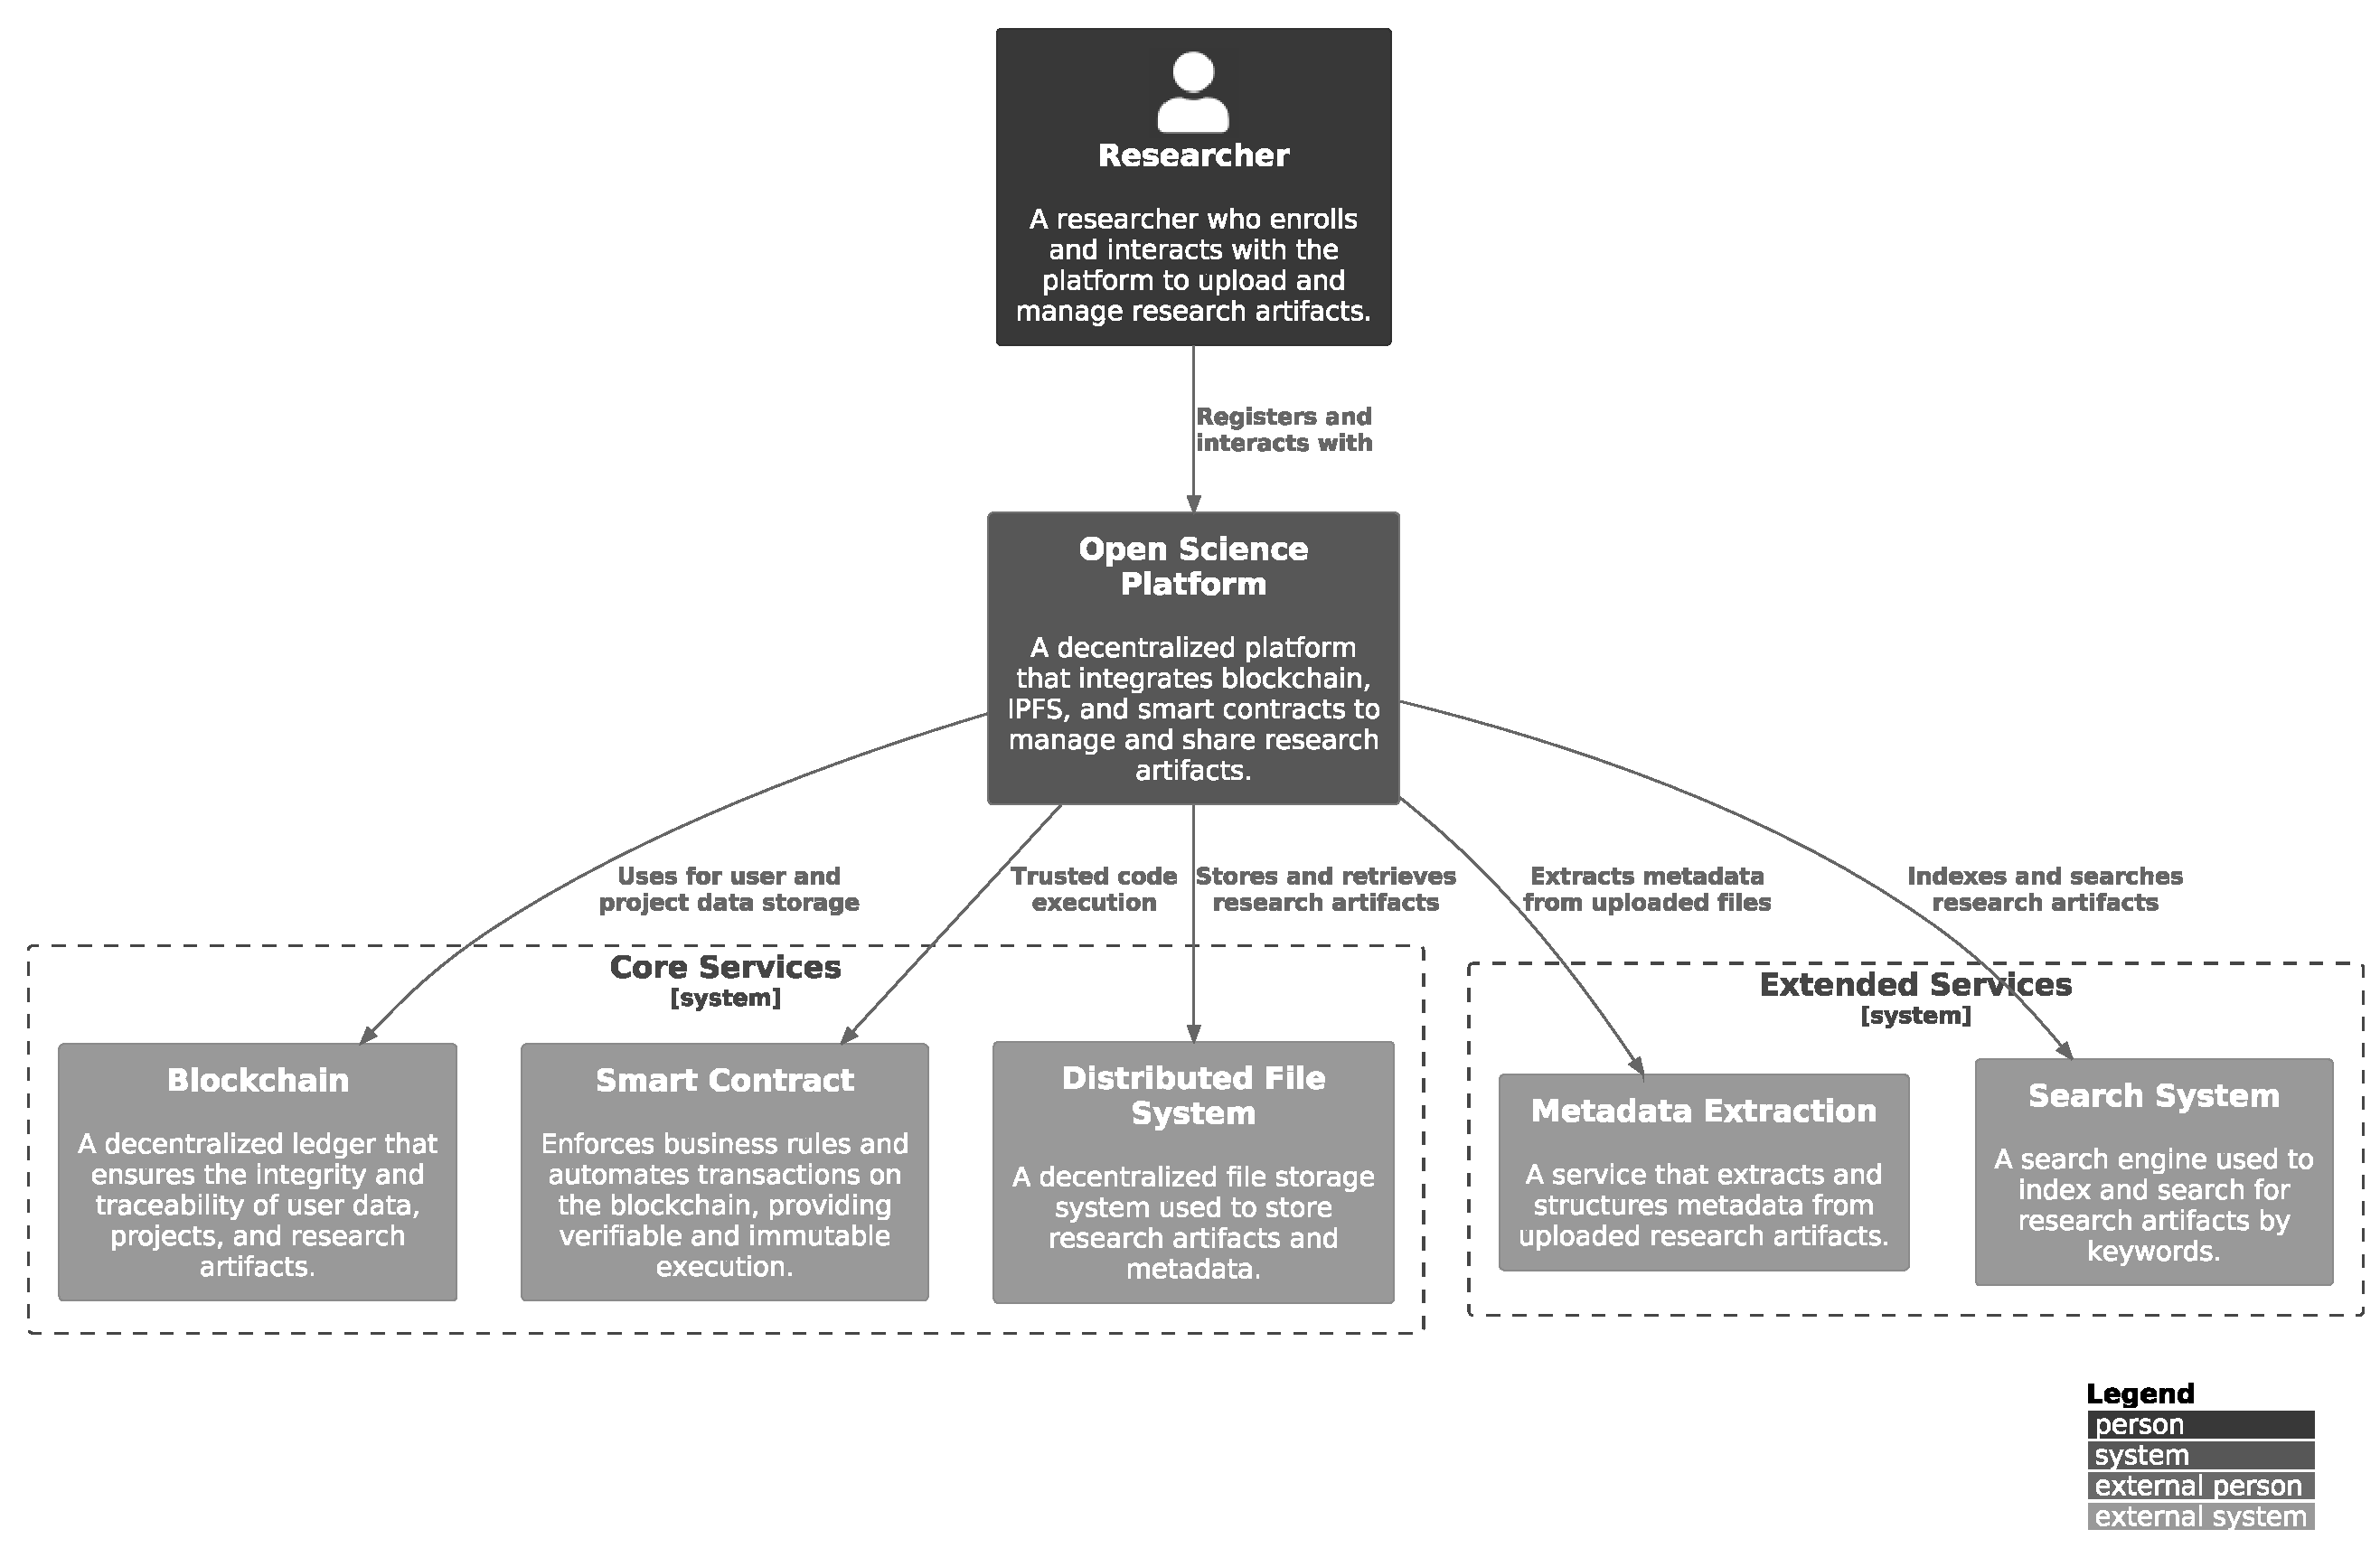
\includegraphics[scale=0.30]{fig/c4_context_diagram.eps}
    \caption{System context diagram}
    \label{fig:c4_context_diagram}
\end{figure}

\subsection{Distributed Trust Architecture}

The d-OSP integrates decentralized and distributed technologies to enhance reproducibility in scientific research. Traditional research infrastructures often suffer from data silos, paywalled access, and risks of data loss or manipulation. By leveraging blockchain and IPFS, the platform ensures that research data remains tamper-proof, permanently accessible, and verifiable.

Researchers can upload experimental protocols, datasets, and publications to the IPFS decentralized network, preventing single points of failure and enabling unrestricted access to research outputs. Blockchain serves as a provenance-tracking mechanism by recording immutable hashes (CIDs) of research data, ensuring the integrity and authenticity of published findings.

Through the integration of these technologies, the d-OSP mitigates the risks associated with centralized control in research dissemination. Traditional repositories may impose restrictions on data access, suffer from institutional biases, or become unavailable over time. In contrast, a decentralized infrastructure empowers researchers to share knowledge freely, ensuring that scientific progress remains transparent and universally accessible.

Decentralization and distributed systems redefine how data integrity, accessibility, and transparency are maintained across various domains. Blockchain and IPFS provide complementary solutions that enhance security, immutability, and scalability. In the context of Open Science, these technologies eliminate reliance on centralized institutions, ensuring that research data remain verifiable and permanently accessible. By leveraging decentralization, the d-OSP fosters an ecosystem of trustless collaboration, where scientific knowledge can be openly shared and validated by the global research community. To fully grasp the impact of these technologies, it is essential to examine their core components and underlying mechanisms. The following sections explore blockchain fundamentals, decentralized applications (dApps), and IPFS, detailing how each contributes to building a resilient and transparent digital infrastructure to enhance science reproducibility.

%====================================================================
\section{Technology Stack}
\label{chp:proposed_model:sec:tech_stack}
%====================================================================

The d-OSP is built on a hybrid architecture that strategically integrates decentralized and centralized components to balance security, traceability, and efficiency in data management. Decentralized technologies, such as blockchain and IPFS, ensure data integrity and tamper resistance, while centralized components facilitate indexing, search, and user interactions. Figure~\ref{fig:c4_container_diagram} presents a high-level breakdown of the platform's core building blocks.

\subsection{Core Services}

The core services of the d-OSP provide the fundamental infrastructure for secure and verifiable research data management.

\begin{itemize}
    \item \textbf{Hyperledger Iroha v1 Blockchain:} Acts as the immutable ledger for managing user and project accounts, recording transactions, and enforcing business rules via smart contracts to ensure secure and transparent data exchange.
    \item \textbf{InterPlanetary File System (IPFS):} Provides decentralized, tamper-proof storage for research files and metadata, ensuring persistent and verifiable access to shared data.
\end{itemize}

\subsection{Extended Services}

The extended services enhance the platform's features by improving file and metadata processing.

\begin{itemize}
    \item \textbf{Apache Tika:} Extracts metadata from uploaded files, enhancing research data organization and search.
    \item \textbf{Whoosh:} Facilitates efficient indexing and keyword-based search for stored files.
\end{itemize}


\subsection{User Interface, integration and execution}

\begin{itemize}
    \item \textbf{Jupyter Notebooks (Python):} Powers the front-end interface, facilitating the automation and display of the execution steps. Blockchain interactions are managed via the Iroha v1 Python library, while communication with the IPFS network is handled through the HTTPS client library.
\end{itemize}

\begin{figure}[htbp]
    \centering
    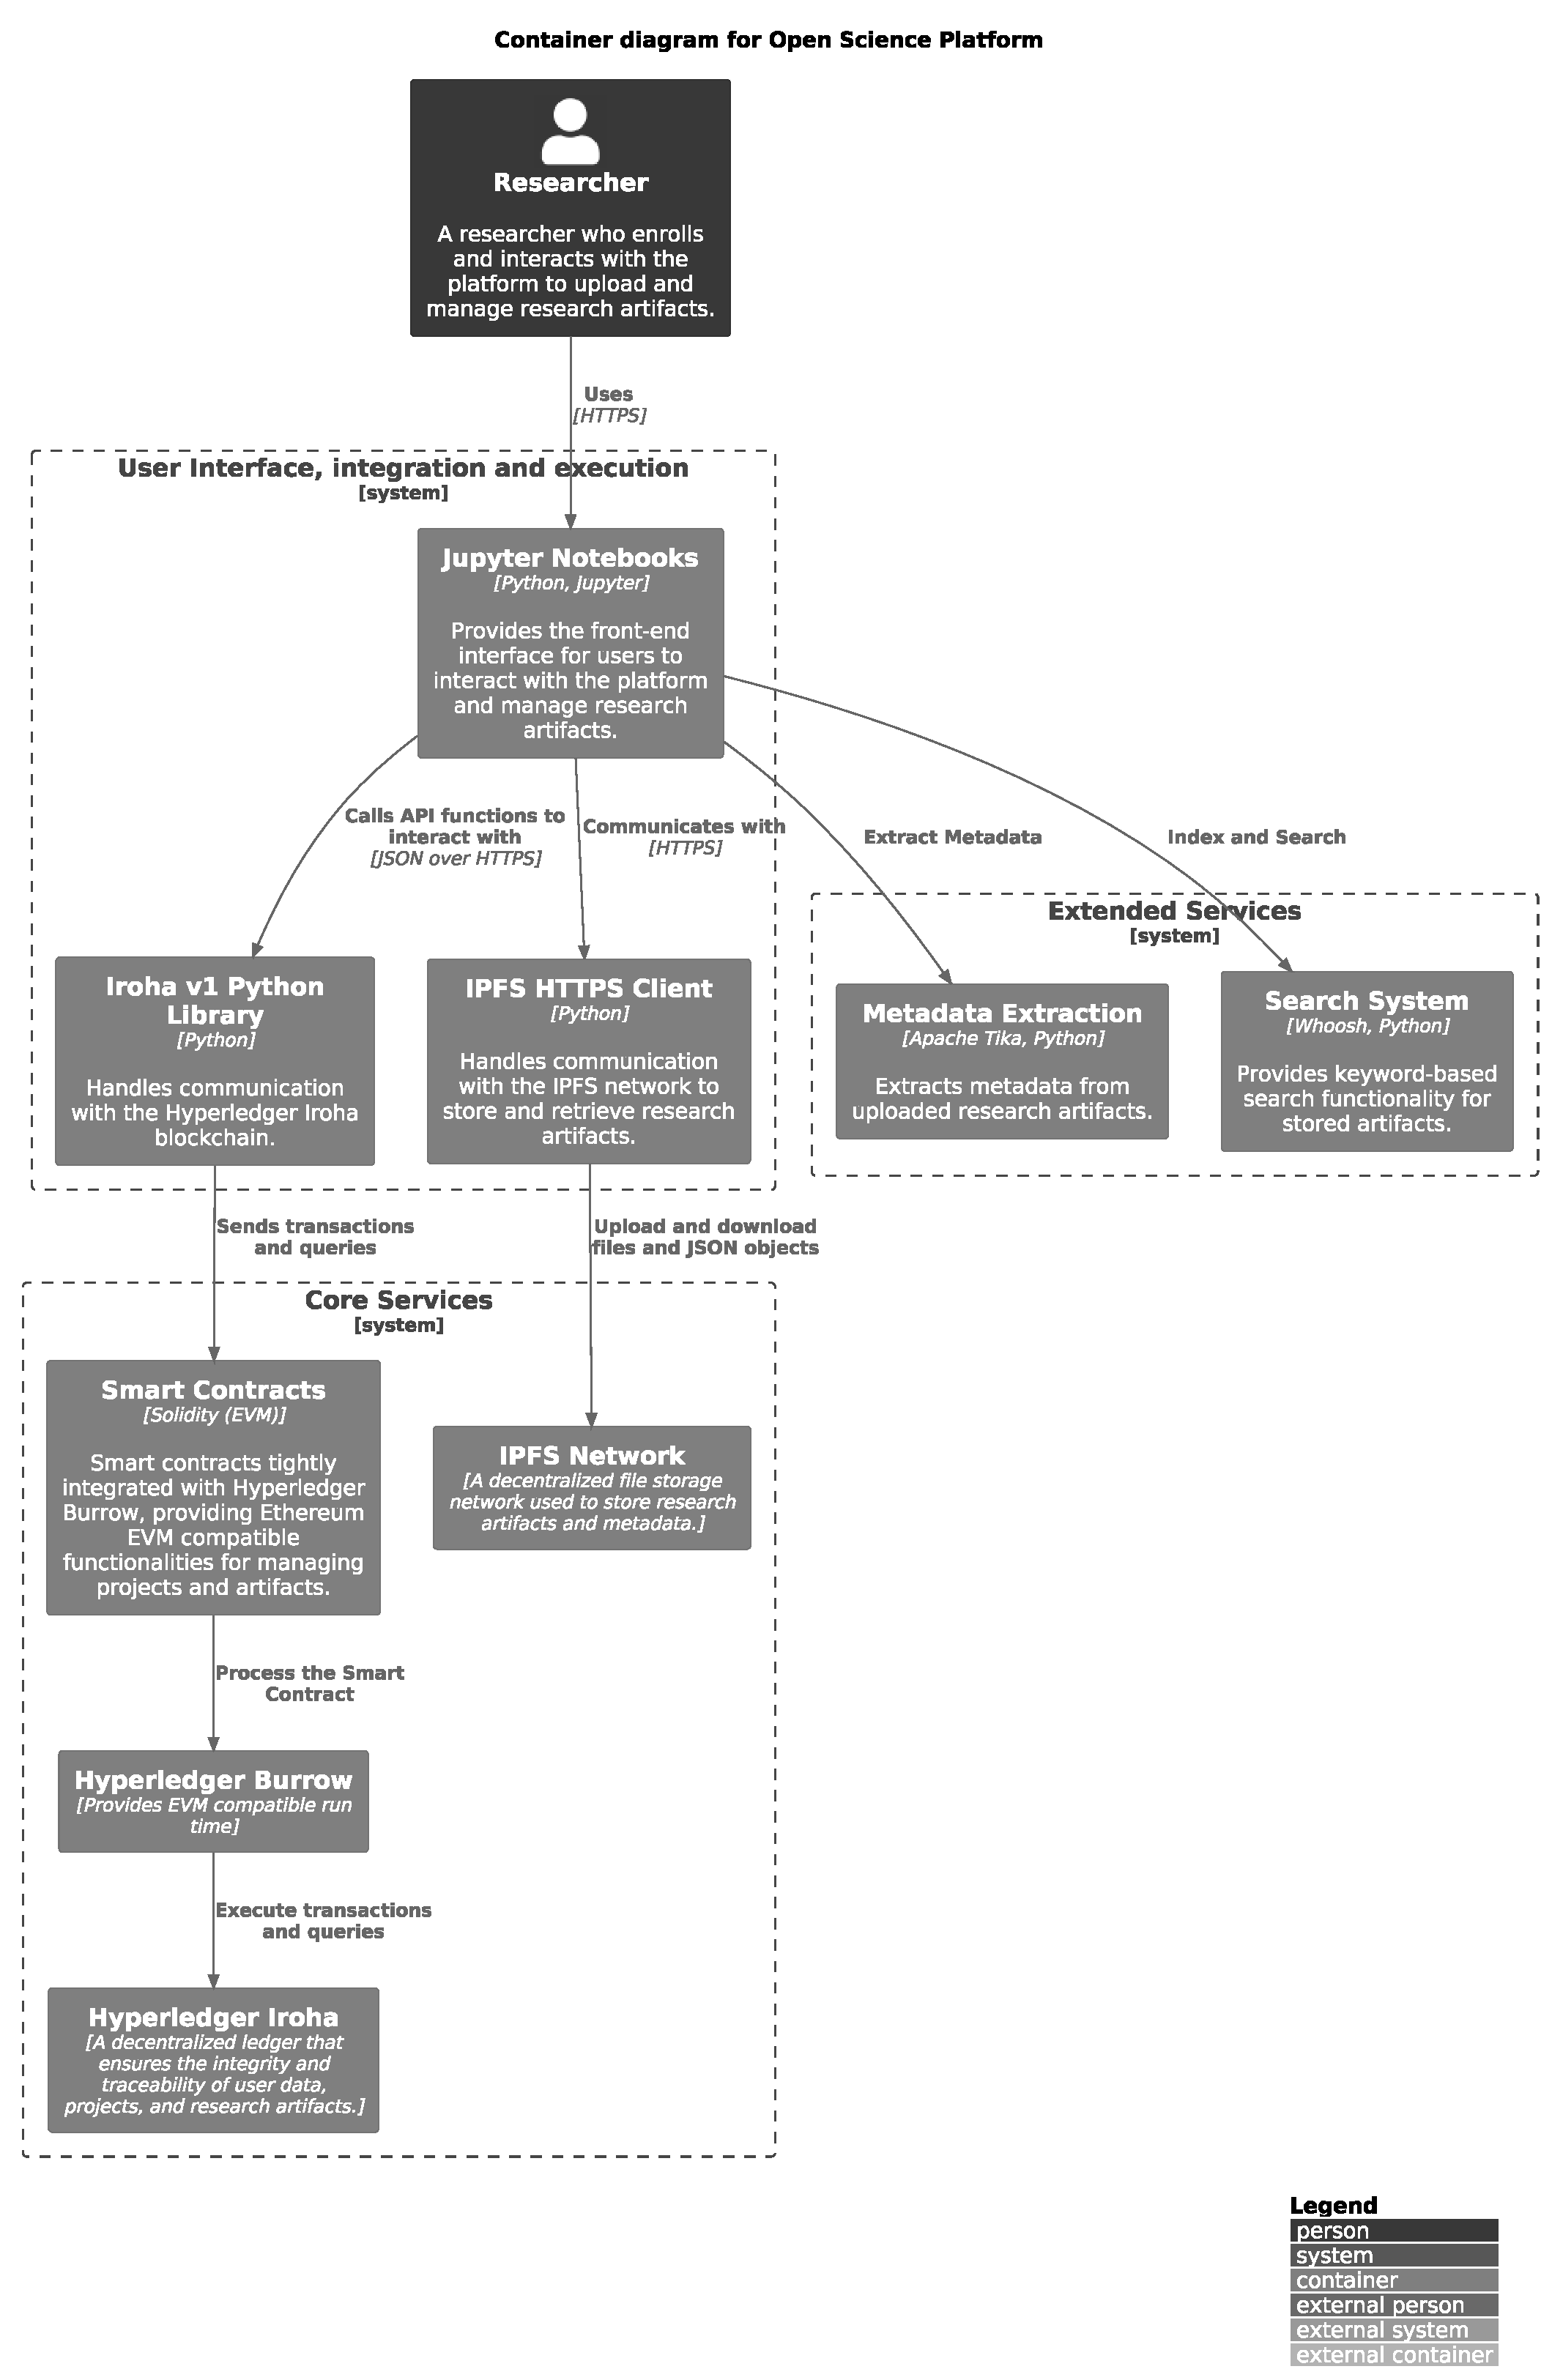
\includegraphics[scale=0.3]{fig/c4_container_diagram.eps}
    \caption{Container diagram}
    \label{fig:c4_container_diagram}
\end{figure}


\subsection{System Components and Interactions}

The d-OSP consists of multiple interconnected components, each serving a distinct role in ensuring secure, verifiable, and reproducible research data management. The primary components include Jupyter Server, the blockchain Hyperledger Iroha v1 and the InterPlanetary File System (IPFS). Each of these elements are encapsulated within a Docker container to provide modularity, ease of deployment and reproducibility. The implementation level architecture is presented in Figure~\ref{fig:c4_component_diagram}, the network topology is depicted in Figure~\ref{fig:docker_ntw_topology}



\begin{figure}[htbp]
    \centering
    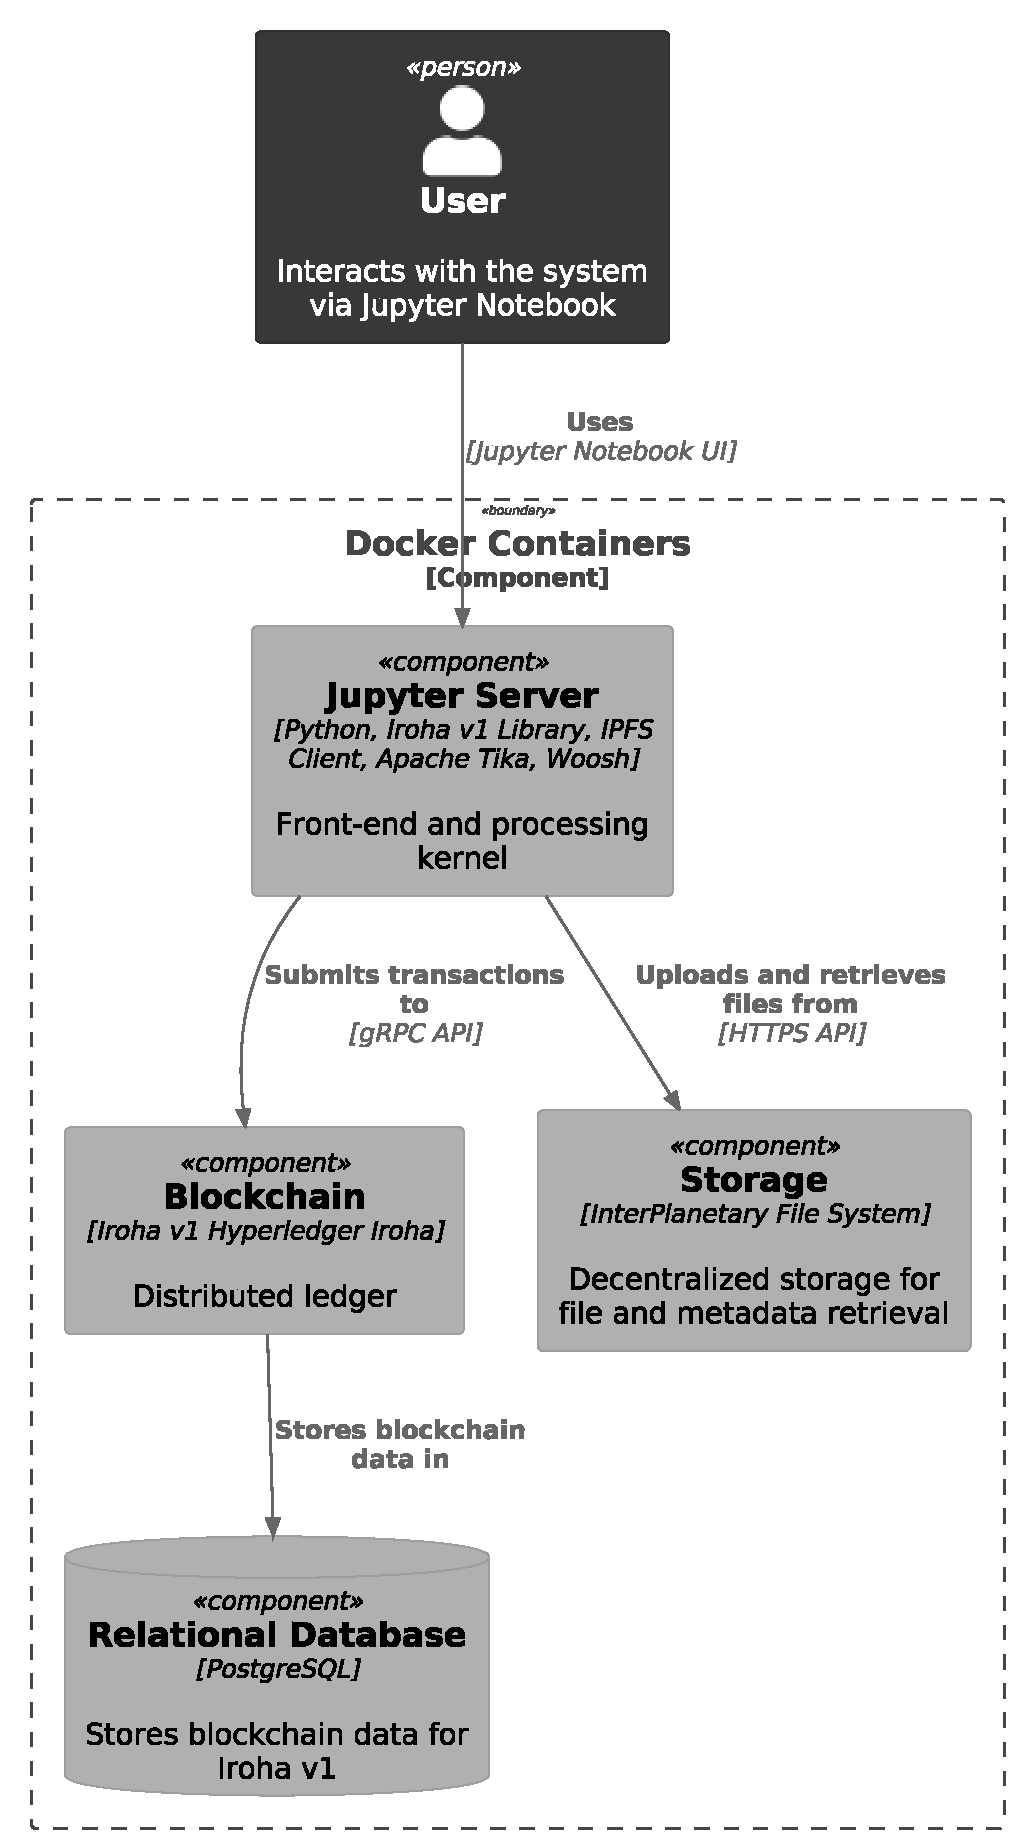
\includegraphics[scale=0.4]{fig/c4_component_diagram.eps}
    \caption{Component diagram}
    \label{fig:c4_component_diagram}
\end{figure}


\begin{figure}[htbp]
    \centering
    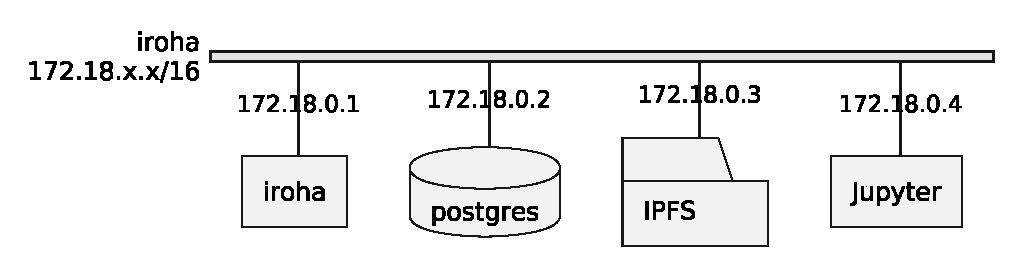
\includegraphics[scale=0.5]{fig/network_topology.eps}
    \caption{Docker network topology}
    \label{fig:docker_ntw_topology}
\end{figure}

\subsubsection{Jupyter Server}
The Jupyter Server acts as the primary interface for users interacting with the platform. This component provides a Python kernel for the execution environment that integrates the Iroha v1 Library, the IPFS HTTPS client, Apache Tika for metadata handling, and the Woosh Indexer and Search system. It enables users to:

\begin{itemize}
    \item Execute Python scripts to submit transactions and queries to the blockchain via smart contracts.
    \item Upload and retrieve files and metadata (JSON objects) stored in IPFS.
    \item Process and index research data using Apache Tika and Woosh for enhanced searchability.
    \item Access and visualize blockchain-stored metadata for Open Science applications.
\end{itemize}

\subsubsection{Blockchain}
The blockchain runs based on a Hyperledger Iroha v1 network and acts as a distributed ledger for recording transactions. It ensures immutability, transparency, and verifiability of stored research metadata. This component:
\begin{itemize}
    \item Receives transactions from the Jupyter Server via a gRPC API.
    \item Stores metadata references, ensuring that uploaded research files can be authenticated.
    \item Interacts with PostgreSQL for structured storage of blockchain metadata.
    \item Supports smart contracts through the integration of Hyperledger Burrow, which provides a modular blockchain client with a permissioned smart contract interpreter partially developed to the specification of the Ethereum Virtual Machine (EVM).

\end{itemize}

\subsubsection{Storage}
The InterPlanetary File System (IPFS) is a decentralized storage solution that manages the research outputs. This component:
\begin{itemize}
    \item Stores digital research files in a content-addressed manner.
    \item Allows the Jupyter Server to upload and retrieve files via an HTTPS API.
    \item Ensures long-term availability of scientific data through distributed storage principles.
\end{itemize}


\subsubsection{Relational Database (PostgreSQL)}
The PostgreSQL database provides structured storage for blockchain-related data. It is used exclusively and managed by Iroha v1 to:
\begin{itemize}
    \item Maintain an efficient and queryable record of transactions.
    \item Ensure that research metadata stored on the blockchain can be retrieved and verified.
    \item Support blockchain operations requiring fast access to structured data.
\end{itemize}

\subsubsection{Component Interactions}
The components interact in aseamless and decentralized manner:
\begin{enumerate}
    \item \textbf{User Interaction}: The user submits transactions, uploads files, and queries research data through the Jupyter Server.
    \item \textbf{Blockchain Transactions}: Jupyter Server sends and retrieves research metadata to the Iroha blockchain via gRPC API.
    \item \textbf{Metadata Storage}: Iroha stores data in the PostgreSQL database for efficient retrieval.
    \item \textbf{Decentralized Storage}: Research files are stored in IPFS, with their unique file identifiers recorded on the blockchain.
    \item \textbf{File Retrieval}: Users can retrieve files from IPFS using their content identifiers (CID), ensuring authenticity and reproducibility.
\end{enumerate}

This architecture guarantees trustworthy and reproducible scientific research by leveraging blockchain for integrity, IPFS for decentralized storage, and Jupyter as an accessible research environment.


%====================================================================
\section{Operations}
\label{chp:proposed_model:sec:operations}
%====================================================================

The platform supports a set of core operations that regulate user interactions with projects and research artifacts.

\subsection{User Enrollment and Project Registration}

\sloppy
The d-OSP enables user enrollment and project registration, ensuring transparent and verifiable account management on the blockchain. Users self-enroll by providing cryptographic credentials and identity details, which are securely stored using a combination of blockchain attributes and decentralized storage through IPFS. Similarly, projects are registered with essential metadata, establishing a distinct blockchain account for each. To maintain traceability and facilitate efficient project management, the system links user and project accounts bidirectionally, allowing for streamlined queries and provenance tracking. These processes are depicted in Figure~\ref{fig:c4_operations_1}.
\fussy

\begin{itemize}
    \item \textbf{User Self-Enrollment} – A user self-enrolls on the platform by providing a private key that complies with the ED25519 or SHA-3 standards and identity information, including full name, institution, email, ORCID, and role. An account is created for the user in the blockchain. All data provided in the enrollment is structured in key/value pairs into a JSON object and uploaded to IPFS, with the corresponding Content Identifier (CID) permanently linking the user’s metadata to their blockchain account.

    \item \textbf{Project Registration} – Users can register a project by specifying a descriptive name, an abstract, relevant keywords, start and end dates, funding agency, and location. Upon registration, a blockchain account is created. This data is structured in key/value pairs into a JSON object and uploaded to IPFS, with the related Content Identifier (CID) ensuring that project-related metadata remains immutable and verifiable within the blockchain.

    \item \textbf{User and Project Accounts Linkage} – Once both user and project accounts are created, the system updates their attributes to establish a bidirectional association. This ensures that querying a user account reveals linked project accounts, and vice versa, facilitating traceability and efficient project management.
\end{itemize}


\begin{figure}[htbp]
    \centering
    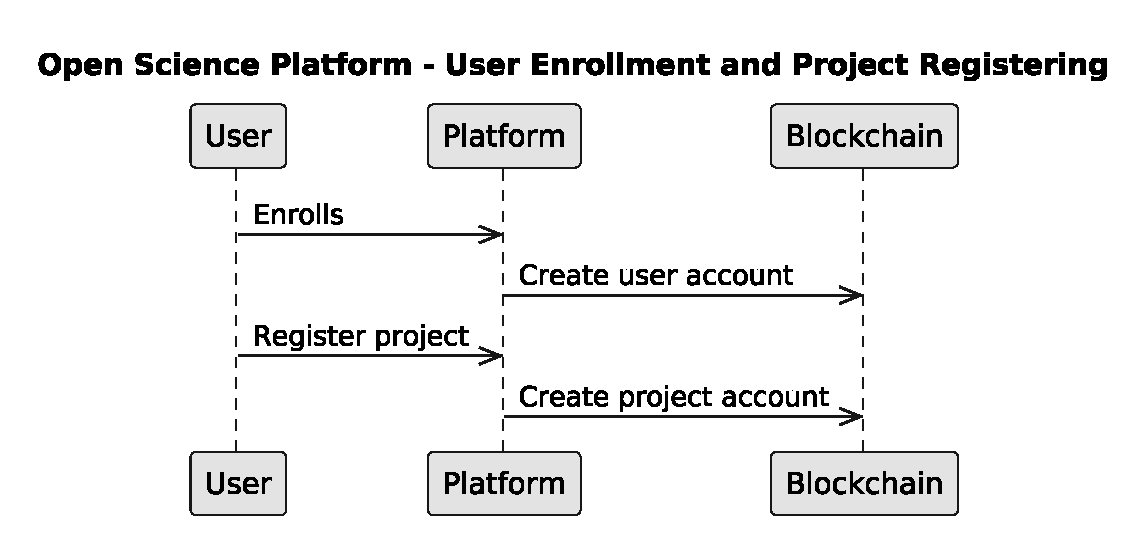
\includegraphics[scale=0.5]{fig/c4_platform_operations_1.eps}
    \caption{User enrollment and project registering}
    \label{fig:c4_operations_1}
\end{figure}

\subsection{Scientific Data Management}

The d-OSP provides a structured approach to managing research data, ensuring their integrity, traceability, and accessibility. Users can upload various types of research files, including papers, datasets, and images, which are securely stored in a decentralized manner using IPFS. Each uploaded file is assigned a unique Content Identifier (CID), which is recorded on the blockchain, creating a tamper-proof reference. To enhance discoverability, the file metadata is extracted, structured, and stored on IPFS, with its CID also registered on the blockchain. The system further supports indexing and full-text search capabilities, enabling efficient retrieval of research files.

The file upload and metadata management workflow are illustrated in Figure~\ref{fig:c4_file_operations_diagram}. A user may upload research files, such as papers, datasets, and images, which are stored on IPFS. Each file is assigned a unique CID, ensuring traceability and integrity, and this CID is recorded on the blockchain attributes of the corresponding project account. After upload, metadata is extracted, structured in key/value pairs, and uploaded to IPFS, with its CID also recorded on the blockchain to preserve provenance. To enhance searchability, the system indexes metadata, including full-text indexing for text-based files.

\begin{figure}[htbp]
    \centering
    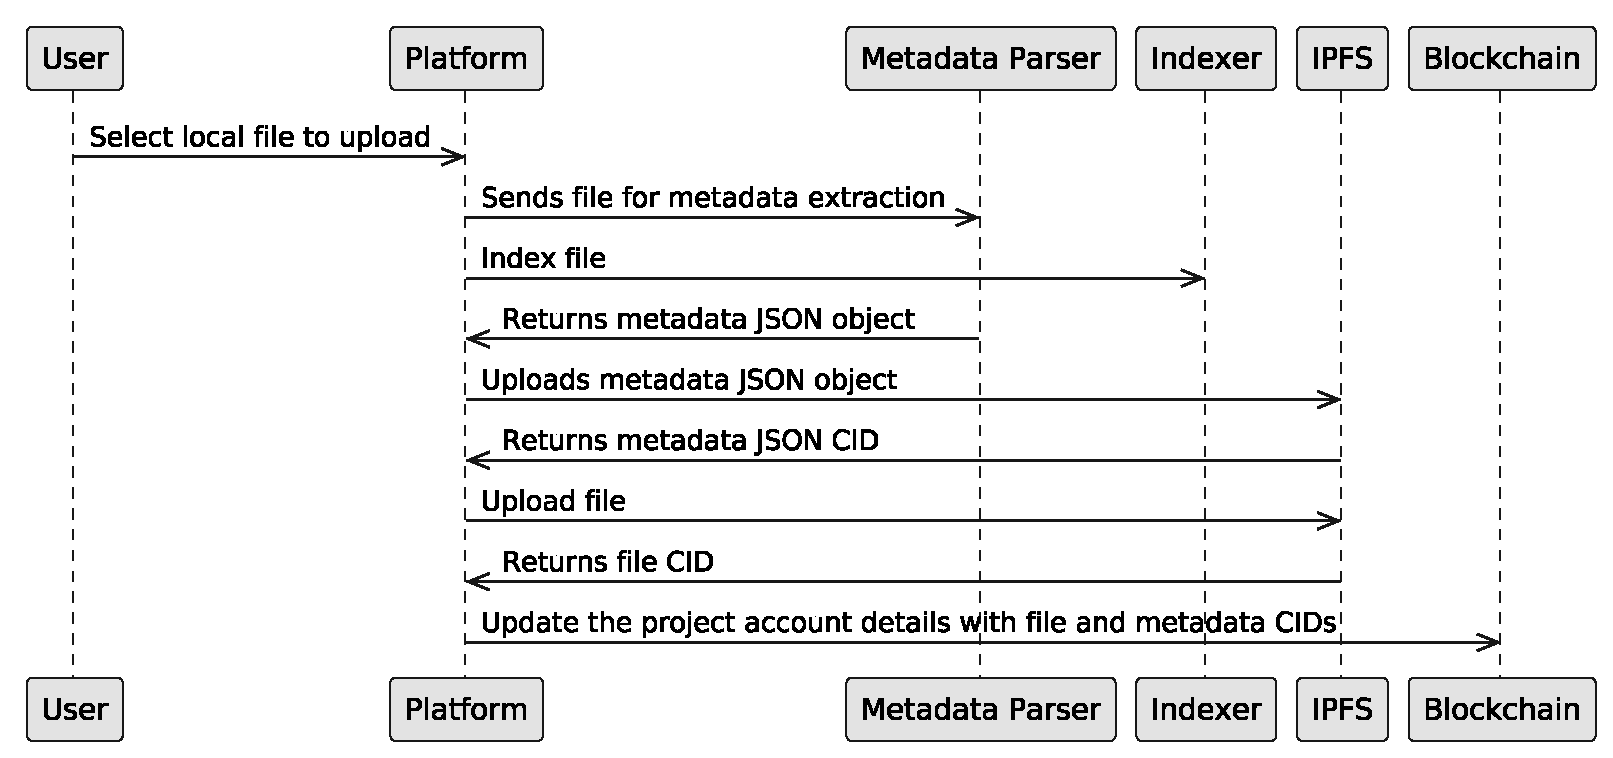
\includegraphics[scale=0.5]{fig/c4_platform_operations_2.eps}
    \caption{File operations diagram}
    \label{fig:c4_file_operations_diagram}
\end{figure}

The platform also enables users to search for research data files using keyword-based queries. As depicted in Figure~\ref{fig:c4_keyword_search}, the search engine looks up keywords in the indexed metadata and returns relevant results. Each result includes metadata details such as descriptions, subjects, and authorship, allowing users to identify relevant files efficiently.

\begin{figure}[htbp]
    \centering
    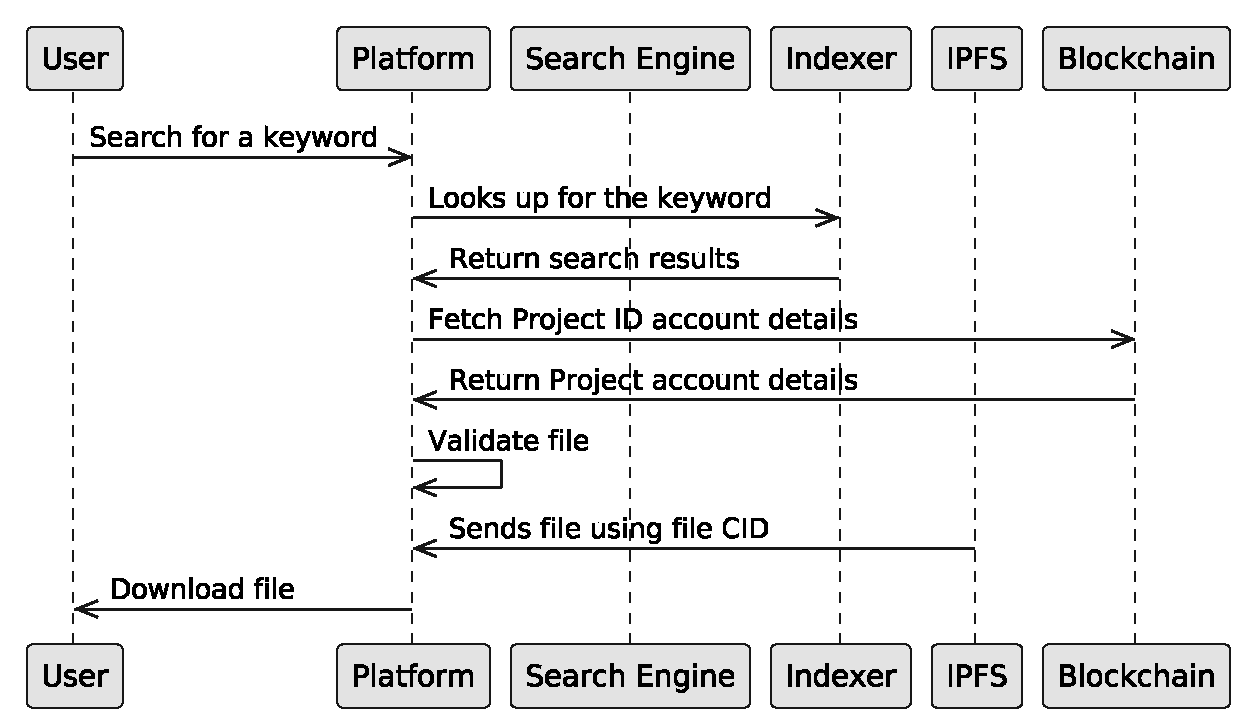
\includegraphics[scale=0.5]{fig/c4_searching_and_validation.eps}
    \caption{Keyword search, file validation, and download}
    \label{fig:c4_keyword_search}
\end{figure}

Once a file has been located, the platform performs a validation step to ensure its integrity and authenticity. The CID stored on IPFS is compared against the CID recorded on the blockchain. If they match, the file is considered valid; otherwise, the system flags it as potentially tampered with or corrupted. This validation mechanism safeguards research data against unauthorized modifications. The file validation and retrieval process is depicted in Figure~\ref{fig:c4_file_validation}. A validated file can then be retrieved and downloaded from IPFS to the user's local system for further use.

\begin{figure}[htbp]
    \centering
    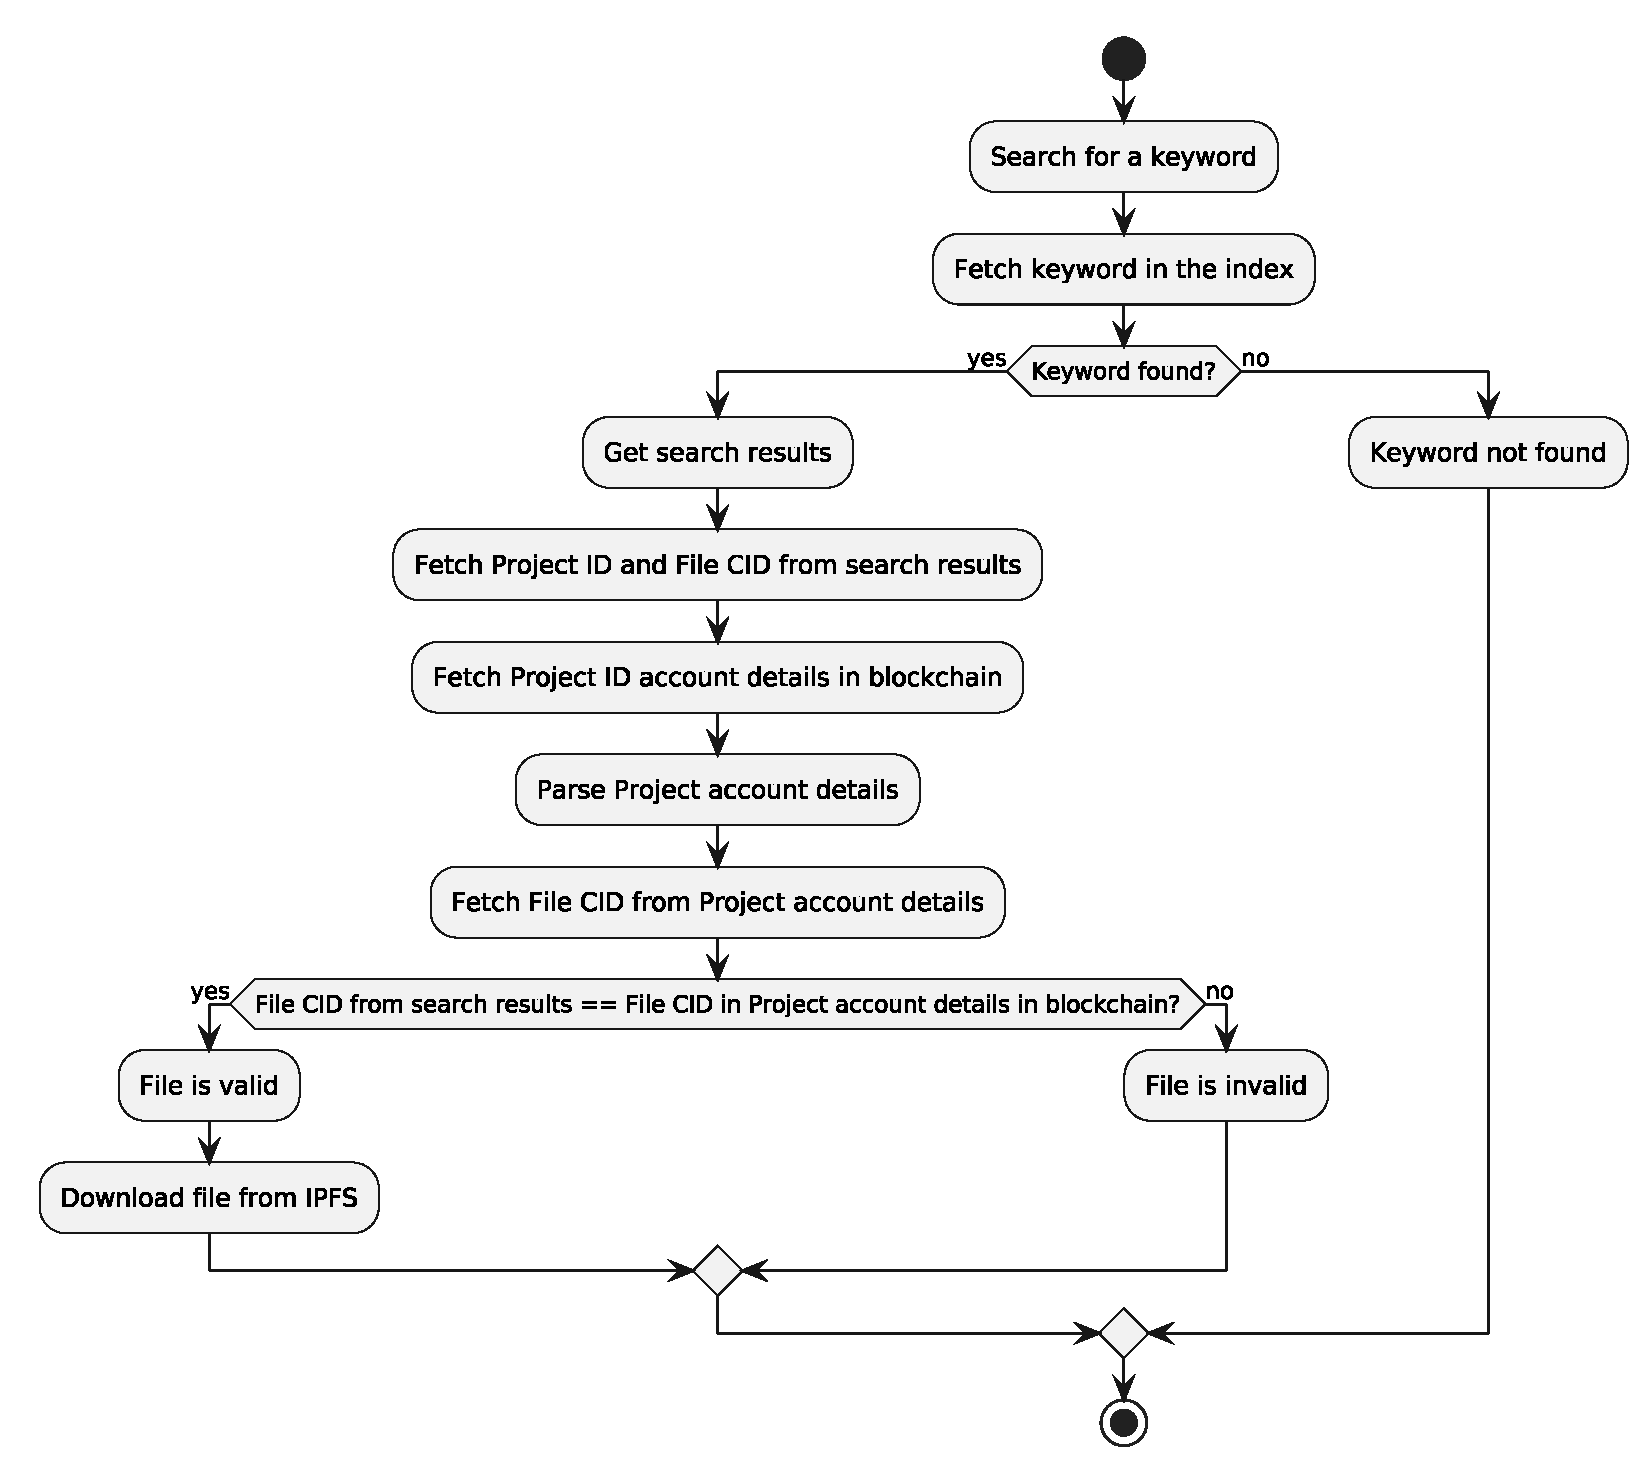
\includegraphics[scale=0.5]{fig/keyword_and_file_validation.eps}
    \caption{File validation and download}
    \label{fig:c4_file_validation}
\end{figure}


%====================================================================
\section{Proposed Data Model}
\label{chp:proposed_model:sec:data_model}
%====================================================================

The entity-relationship model for the d-OSP defines the logical structure of users and research projects, capturing the associations between these entities. The primary entities in this model are \texttt{User} and \texttt{Project}, which are connected through a linked relationship, Figure~\ref{fig:er_model} presents the model.


\begin{figure}[htbp]
    \centering
    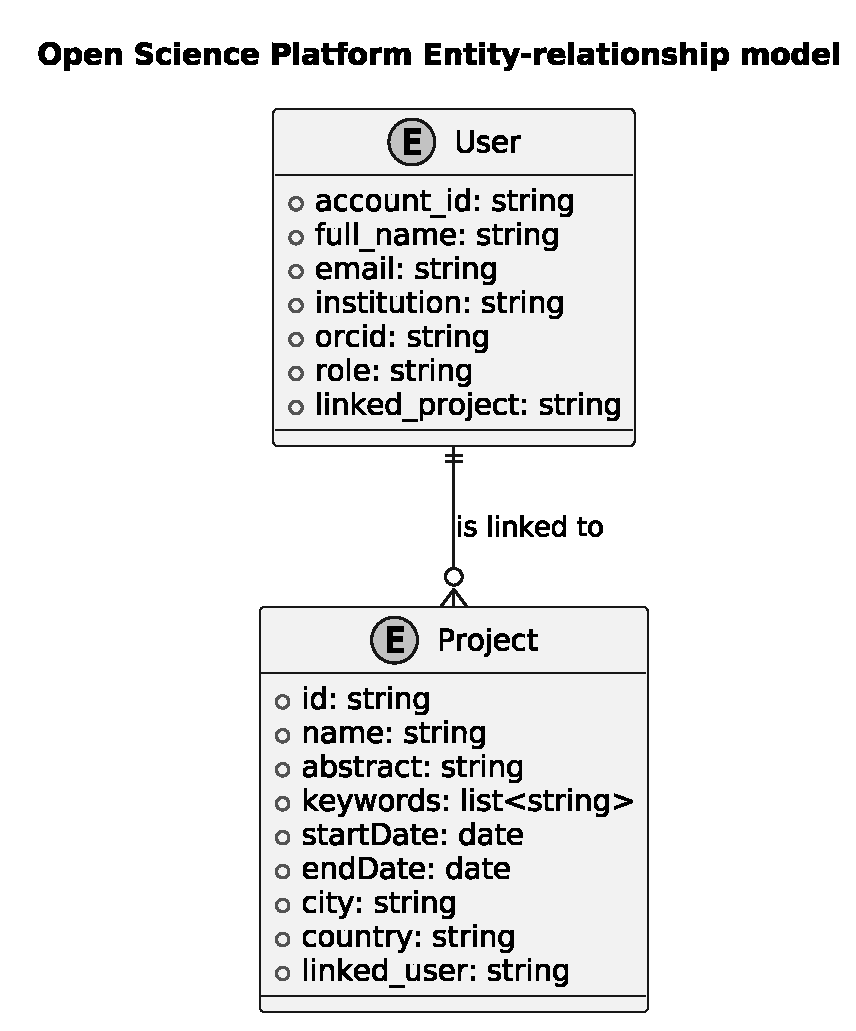
\includegraphics[scale=0.5]{fig/entity_relationship_model.eps}
    \caption{Entity-relationship model}
    \label{fig:er_model}
\end{figure}



\subsection{User Entity}
The \texttt{User} entity represents an individual interacting with the platform. Each user is uniquely identified by an account ID and has attributes that describe personal and institutional information. The attributes of the \texttt{User} entity are listed in Table \ref{tab:user_entity}.

\begin{table}[h]
    \centering
    \renewcommand{\arraystretch}{1.2}
    \caption{User Entity Attributes}
    \label{tab:user_entity}
    \begin{tabularx}{\textwidth}{|l|X|}
        \hline
        \textbf{Attribute}       & \textbf{Description}                              \\ \hline
        \texttt{account\_id}     & A unique identifier assigned to the user.         \\ \hline
        \texttt{full\_name}      & The complete name of the user.                    \\ \hline
        \texttt{email}           & The email address used for communication.         \\ \hline
        \texttt{institution}     & The organization to which the user is affiliated. \\ \hline
        \texttt{orcid}           & The Open Researcher and Contributor ID.           \\ \hline
        \texttt{role}            & The role of the user within the research project. \\ \hline
        \texttt{linked\_project} & The research project the user is assigned to.     \\ \hline
    \end{tabularx}
\end{table}


\subsection{Project Entity}
The \texttt{Project} entity represents a research project registered in the platform. It contains essential metadata to describe the project and facilitate discovery and collaboration. The attributes of the \texttt{Project} entity are listed in Table \ref{tab:project_entity}.

\begin{table}[h]
    \centering
    \renewcommand{\arraystretch}{1.2}
    \caption{Project Entity Attributes}
    \label{tab:project_entity}
    \begin{tabularx}{\textwidth}{|l|X|}
        \hline
        \textbf{Attribute}    & \textbf{Description}                                                \\ \hline
        \texttt{project\_id}  & A unique identifier assigned to the project.                        \\ \hline
        \texttt{name}         & The official name of the project.                                   \\ \hline
        \texttt{abstract}     & A brief summary outlining the research objectives.                  \\ \hline
        \texttt{keywords}     & A list of relevant keywords associated with the project.            \\ \hline
        \texttt{startDate}    & The date when the project officially begins.                        \\ \hline
        \texttt{endDate}      & The date when the project was concluded or is expected to conclude. \\ \hline
        \texttt{city}         & The city where the project is primarily conducted.                  \\ \hline
        \texttt{country}      & The country associated with the research project.                   \\ \hline
        \texttt{linked\_user} & The user linked to the project.                                     \\ \hline
    \end{tabularx}
\end{table}


\subsection{Linked Entities}

A \texttt{User} is linked to one or more \texttt{Project} entities, establishing a one-to-many relationship. This means that a single user can be associated with multiple projects. This model ensures a structured representation of research projects and their linked users, supporting an organized approach to data management in the d-OSP.

%====================================================================
\section{Hyperledger Iroha Data Model }
\label{chp:proposed_model:sec:iroha_data_model}
%====================================================================


The entity-relationship (ER) model of Hyperledger Iroha defines the core entities, attributes, and relationships that facilitate role-based access control, asset management, and multi-signature security. While Iroha v1 includes a broader set of entities, this research focuses solely on the account and domain related classes and attributes, as presented in Figure~\ref{fig:iroha_v1_er_model}

\subsection{Account Entity}
The \texttt{account} entity represents a user or system account registered on the blockchain. Table \ref{tab:account_entity} lists its attributes.

\begin{table}[h]
    \centering
    \renewcommand{\arraystretch}{1.2}
    \caption{Attributes of the \texttt{account} entity}
    \label{tab:account_entity}
    \begin{tabularx}{\textwidth}{|l|X|}
        \hline
        \textbf{Attribute}   & \textbf{Description}                                            \\ \hline
        \texttt{account\_id} & Unique identifier of the account                                \\ \hline
        \texttt{domain\_id}  & Links the account to a specific domain                          \\ \hline
        \texttt{quorum}      & Required number of signatories for multi-signature transactions \\ \hline
        \texttt{data}        & Stores additional metadata in JSON format                       \\ \hline
    \end{tabularx}
\end{table}


\subsection{Domain Entity}
The \texttt{domain} entity organizes accounts within logical boundaries. A \texttt{domain} can contain multiple \texttt{accounts}, as illustrated in Table~\ref{tab:domain_entity}.

\begin{table}[h]
    \centering
    \renewcommand{\arraystretch}{1.2}
    \caption{Attributes of the \texttt{domain} entity}
    \label{tab:domain_entity}
    \begin{tabularx}{\textwidth}{|l|X|}
        \hline
        \textbf{Attribute}     & \textbf{Description}                                        \\ \hline
        \texttt{domain\_id}    & Unique identifier for the domain                            \\ \hline
        \texttt{default\_role} & Default role assigned to accounts created within the domain \\ \hline
    \end{tabularx}
\end{table}



\begin{figure}[htbp]
    \centering
    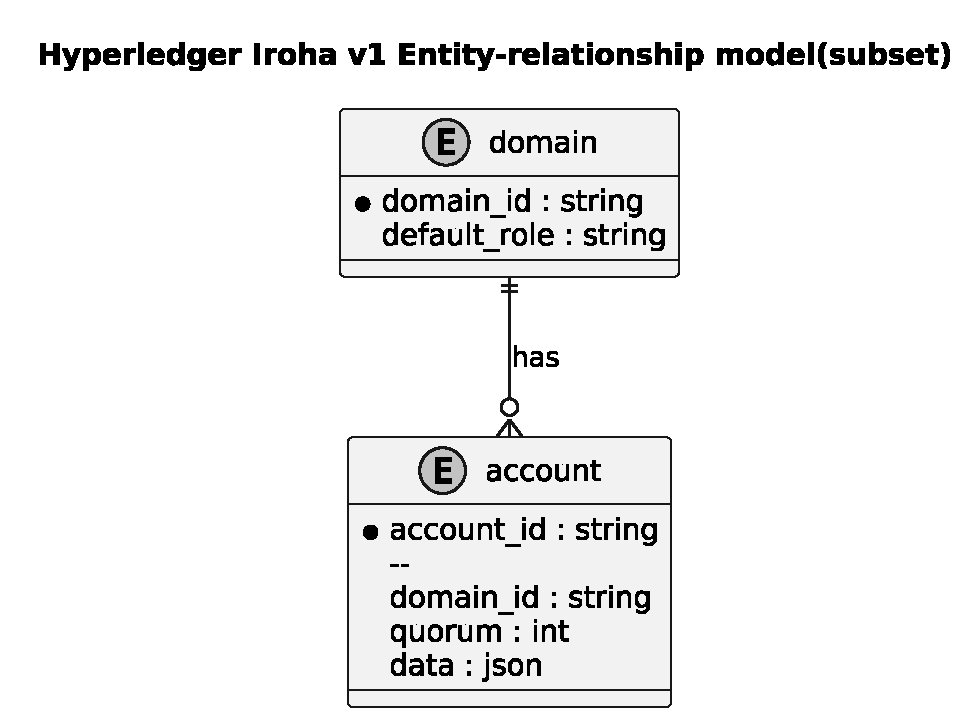
\includegraphics[scale=0.5]{fig/iroha_v1_er_model.eps}
    \caption{Subset of the Iroha v1 Entity-relationship model}
    \label{fig:iroha_v1_er_model}
\end{figure}


This ER model follows Hyperledger Iroha’s permissioned blockchain structure. It ensures fine-grained access control, multi-signature security, and domain-based account management.


%====================================================================
\section{Relationship Between Models}
\label{chp:proposed_model:sec:iroha_data_model}
%====================================================================

The d-OSP ER model leverages the entity structure of the Iroha v1 ER model, particularly the \texttt{account} entity, to represent both the \texttt{User} and \texttt{Project} entities. In this approach, instead of introducing separate entitties for users and projects, the \texttt{account} entity in the Iroha v1 ER model serves as a general-purpose representation, encapsulating all necessary attributes in a structured format.

The attributes specific to users and projects, which are not natively present in the Iroha v1 \texttt{account} entity, are stored as JSON objects within the \texttt{data} field of the \texttt{account} entity. This design provides a flexible and scalable means of extending the entity's attributes without modifying the core schema of the Iroha blockchain.

From a relational perspective, the \texttt{account} entity maintains its standard associations with roles, permissions, and assets as defined in the Iroha v1 ER model. This ensures that user accounts and project accounts can both participate in the blockchain's permissioning system, asset ownership model, and role-based access control without requiring modifications to the underlying structure.

By reusing the \texttt{account} entity, the d-OSP ER model ensures compatibility with Iroha's existing mechanisms for identity management, cryptographic signing, and permission delegation. Additionally, this approach aligns with the decentralized and immutable nature of blockchain, ensuring that both user and project entities benefit from the security and transparency features inherent to the Iroha v1 framework. Figure~\ref{fig:comparing_er_models} provides a comparison between models and the rationale of use.



\begin{figure}[htbp]
    \centering
    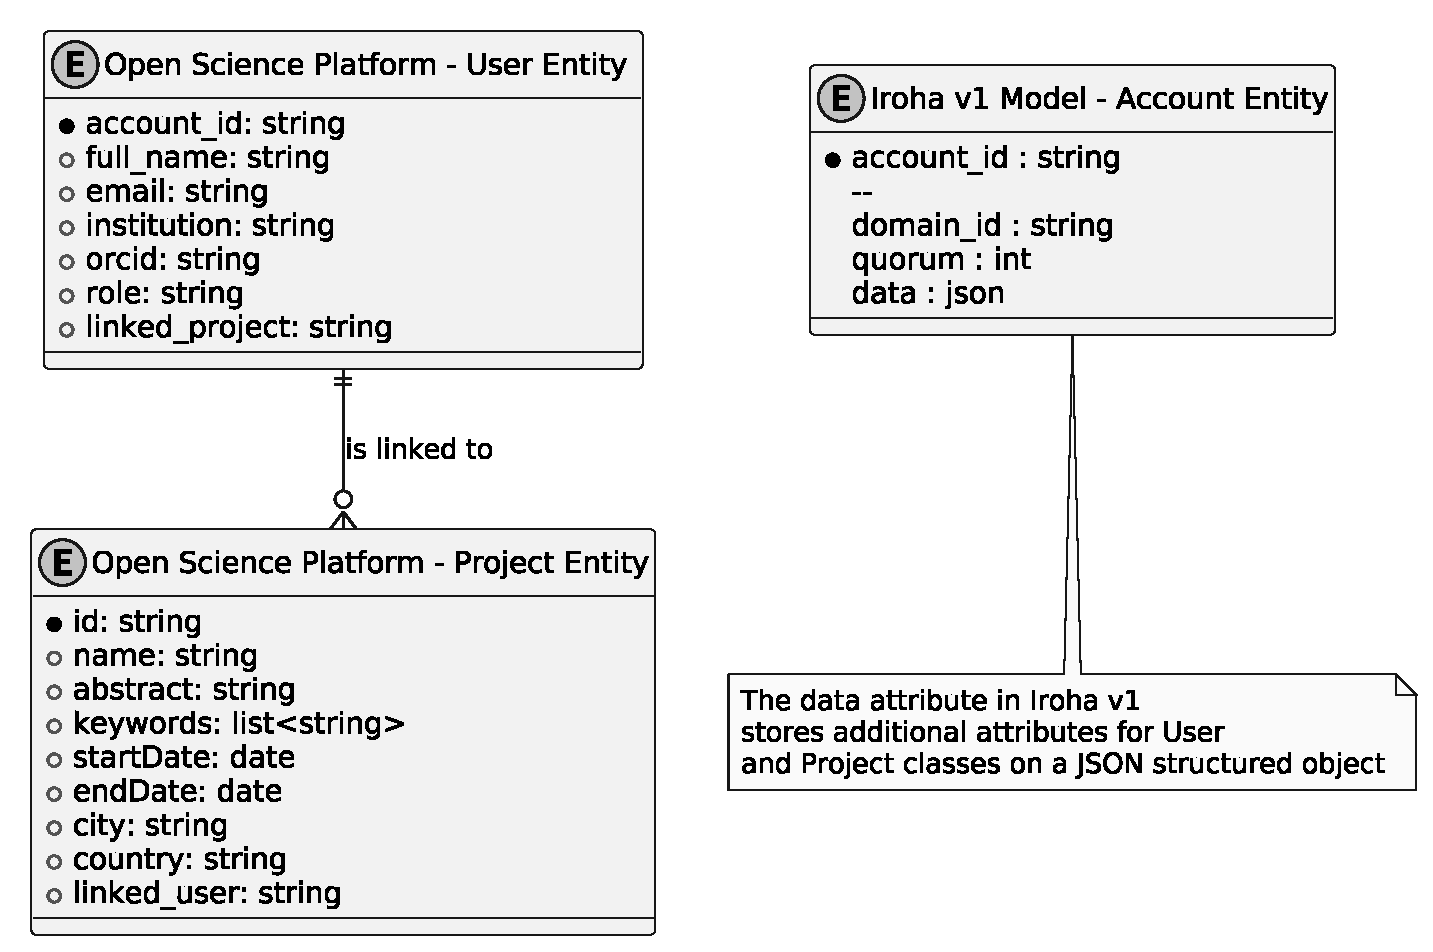
\includegraphics[scale=0.5]{fig/comparing_er_models.eps}
    \caption{Comparison of the Entitiy-relationship models}
    \label{fig:comparing_er_models}
\end{figure}

%====================================================================
\section{Metadata and Ontologies}
\label{chp:proposed_model:sec:ontologies}
%====================================================================

Metadata plays a crucial role in both the \texttt{Account} and \texttt{Project} classes within the d-OSP. It is used to capture and represent essential attributes about the user and the research project, providing context and structure to their respective data. The metadata is stored as JSON objects, following established semantic web 2.0 standards and leveraging ontologies to enhance data interoperability and accessibility.

\subsection{Ontologies}

An ontology is a formal representation of knowledge as a set of concepts within a domain and the relationships between those concepts. Ontologies help structure data in a way that promotes interoperability, consistency, and clarity. The use of ontologies such as \texttt{FOAF}, \texttt{Schema.org}, and \texttt{Dublin Core} ensures that data is standardized and can be easily shared and understood across different systems. These ontologies were selected because of their widespread adoption, their ability to standardize data across different systems, and their support for rich, machine-readable representations.

\begin{table}[h]
    \centering
    \renewcommand{\arraystretch}{1.2}
    \begin{tabularx}{\textwidth}{|l|X|}            \hline
        \textbf{Ontology}                  & \textbf{Description}                                                                                                                                                                                                                                   \\ \hline
        \textbf{FOAF (Friend of a Friend)} & A vocabulary used to describe people, their activities, and their relationships to other people and objects. It is used to describe the \texttt{User} entity, including attributes like name, email, and organization.                                 \\ \hline
        \textbf{Schema.org}                & A collaborative initiative that provides a structured vocabulary for data markup on the web. It is used for describing both \texttt{User} and \texttt{Project} metadata, ensuring compatibility with web standards and promoting data discoverability. \\ \hline
        \textbf{Dublin Core (DC)}          & A metadata standard used for describing a wide range of resources, for describing the abstract, keywords, and other descriptive elements of the \texttt{Project} entity.                                                                               \\ \hline
    \end{tabularx}
    \caption{Ontologies}
    \label{tab:ontologies}
\end{table}


As shown in table~\ref{tab:ontologies}, by aligning with these ontologies, the platform ensures that its metadata is compatible with other Open Science initiatives and services, facilitating seamless integration and data exchange.

%====================================================================
\section{Storing User and Project Attributes}
\label{chp:proposed_model:sec:metadata}
%====================================================================

The two core entities, user and project, are tightly integrated with the blockchain and IPFS through metadata structures. This coupling enables persistent identification, traceability, and contextualization of scientific assets across the platform.


\subsection{User Metadata}

The metadata for the \texttt{Account} class describes the attributes associated with a user on the platform. This metadata is structured using multiple ontologies, primarily \texttt{FOAF} (Friend of a Friend) and \texttt{Schema.org}, to provide detailed and interoperable information about the user. The key attributes in the \texttt{Account} metadata include the user's name, email, organizational affiliation, unique identifier (ORCID), role, public key, and linked project.

\begin{table}[h]
    \centering
    \renewcommand{\arraystretch}{1.2}
    \begin{tabularx}{\textwidth}{|l|X|}
        \hline
        \textbf{Attribute}              & \textbf{Description}                                                                                            \\ \hline
        \texttt{foaf:name}              & The name of the user.                                                                                           \\ \hline
        \texttt{foaf:mbox}              & The email address of the user.                                                                                  \\ \hline
        \texttt{foaf:organization}      & The organization the user is affiliated with, described as an instance of the \texttt{foaf:Organization} class. \\ \hline
        \texttt{schema:identifier}      & A unique identifier for the user, such as an ORCID identifier.                                                  \\ \hline
        \texttt{foaf:holdsAccount}      & The user's account details, including their role and public key.                                                \\ \hline
        \texttt{schema:linked\_project} & The project associated with the user.                                                                           \\ \hline
    \end{tabularx}
    \caption{Account Metadata Attributes}
    \label{tab:user_metadata}
\end{table}

As presented in Table~\ref{tab:user_metadata}, this structured metadata helps ensure the user information is standardized and interoperable across different systems and platforms.


\subsection{Metadata representation}

JSON for Linked Data (JSON-LD) is a lightweight Linked Data format designed to structure and interconnect data on the web using standard JSON. It extends JSON by incorporating semantic web principles, making data more discoverable, reusable, and machine-readable. JSON-LD achieves this by including a \texttt{@context} element, which maps terms to well-defined ontologies, and a \texttt{@graph} element, which structures entities and their relationships in a linked data format.

A key advantage of JSON-LD is its compatibility with existing JSON-based systems while enabling seamless integration with the semantic web. By leveraging vocabularies such as Schema.org and Dublin Core, JSON-LD ensures interoperability across diverse platforms and datasets. This makes it particularly useful for Open Science applications, where structured metadata enhances research reproducibility and data sharing.

In the context of the d-OSP, JSON-LD is used to encode metadata for users and research projects, ensuring alignment with widely accepted ontologies. The structured representation enables automatic indexing, metadata enrichment, and semantic search capabilities, facilitating better knowledge discovery and integration within the scientific community.


\subsection{The User Metadata}

The user metadata is structured using two primary ontologies: Friend of a Friend (FOAF) and Schema.org.

The FOAF ontology is used to describe personal and organizational attributes of users within the platform. It provides well-defined properties such as \texttt{foaf:name} for the user’s full name, \texttt{foaf:mbox} for email addresses, and \texttt{foaf:organization} for institutional affiliations. By leveraging FOAF, the platform ensures standardized representation of user identities and their associations, facilitating integration with other systems that utilize FOAF-based user profiles.

Schema.org complements FOAF by enriching the user metadata with structured properties that enhance discoverability and machine readability. The \texttt{schema:identifier} property, for instance, is used to store unique user identifiers such as ORCID, ensuring compatibility with global researcher identification systems. Additionally, \texttt{schema:roleName} captures the user’s role within the platform (e.g., reviewer, publisher), while \texttt{schema:publicKey} stores cryptographic keys associated with the user’s account. The \texttt{schema:linked\_project} property establishes connections between users and their associated research projects, enabling efficient metadata retrieval and knowledge graph construction as exhibited in Figures~\ref{jsonld:user}, the JSON-LD structure represents the project metadata in the d-OSP.

\begin{listing}
    \begin{minted}[linenos=false,
               xleftmargin=21pt,
               tabsize=4,
               breaklines=true,
               breakanywhere=true]{json}
  {
      "@context": {
          "schema": "http://schema.org/",
          "foaf": "http://xmlns.com/foaf/0.1/"
      },
      "@graph": [
          {
              "@type": "foaf:Person",
              "foaf:name": "Zealous Ptolemy",
              "foaf:mbox": "zealous_ptolemy@email.com",
              "foaf:organization": {
                  "@type": "foaf:Organization",
                  "foaf:name": "Ashkelon Academic College"
              },
              "schema:identifier": {
                  "@type": "PropertyValue",
                  "propertyID": "ORCID",
                  "value": "6153-7096-0437-X"
              },
              "foaf:holdsAccount": {
                  "schema:identifier": "zealous_ptolemy@test",
                  "schema:roleName": "reviewer",
                  "schema:publicKey": "ca4c00c0a43bbd2caf070ab780886906ebb70e2c3d975972ccab4e15c01f33bd"
              },
              "schema:linked_project": "02226@test"
          }
      ]
  }
  
\end{minted}
    \caption{User Metadata}
    \label{jsonld:user}
\end{listing}


By combining FOAF and Schema.org, the d-OSP ensures that user metadata is both human-readable and machine-actionable, promoting seamless integration with external research infrastructures and fostering an interoperable ecosystem for Open Science.

\subsection{The Project Metadata}

The metadata for the \texttt{Project} entity provides essential details about the research project hosted on the platform. Similar to the \texttt{User} metadata, the project metadata is structured using \texttt{Schema.org} and \texttt{Dublin Core} (\texttt{dc}) ontologies. This structure allows for a comprehensive description of the project, including its name, abstract, keywords, timeline, funding details, and location.

\begin{table}[h]
    \centering
    \label{tab:project_metadata}
    \renewcommand{\arraystretch}{1.2}
    \begin{tabularx}{\textwidth}{|l|X|}
        \hline
        \textbf{Attribute}           & \textbf{Description}                                                                                           \\ \hline
        \texttt{schema:name}         & The name of the research project.                                                                              \\ \hline
        \texttt{dc:abstract}         & A brief abstract describing the project's objectives and focus.                                                \\ \hline
        \texttt{schema:keywords}     & Keywords associated with the project, such as "precision agriculture" and "global supply chains."              \\ \hline
        \texttt{schema:startDate}    & The start date of the project.                                                                                 \\ \hline
        \texttt{schema:endDate}      & The end date of the project.                                                                                   \\ \hline
        \texttt{schema:funding}      & The funding organization for the project, described as an instance of the \texttt{schema:Organization} class.  \\ \hline
        \texttt{schema:location}     & The physical location where the project is based, described as an instance of the \texttt{schema:Place} class. \\ \hline
        \texttt{schema:metadataCID}  & A unique identifier for the metadata of the project.                                                           \\ \hline
        \texttt{schema:linked\_user} & The user associated with the project.                                                                          \\ \hline
    \end{tabularx}
    \caption{Project Metadata Attributes}
\end{table}

The following JSON structure describes the metadata for a \texttt{Project} in the d-OSP as shown in Figures~\ref{jsonld:project}.


\begin{listing}
    \begin{minted}[linenos=false,
               xleftmargin=21pt,
               tabsize=4,
               breaklines=true,
               breakanywhere=true]{json}
    {
      "@context": {
          "schema": "http://schema.org/",
          "dc": "http://purl.org/dc/terms/"
      },
      "@graph": [
          {
              "@type": "schema:ResearchProject",
              "schema:identifier": "02226@test",
              "schema:publicKey": "1c6b8d00c8382c93eb0dd3eeb24a20bfece56a28326bbaebb647cadaf4750520",
              "schema:description": {
                  "@context": {
                      "schema": "http://schema.org/",
                      "dc": "http://purl.org/dc/terms/"
                  },
                  "@type": "schema:ResearchProject",
                  "schema:name": "Assessing the Benefits of precision agriculture for global supply chains",
                  "dc:abstract": "This research focuses on the benefits and challenges posed by precision agriculture for global supply chains, with an emphasis on its potential for disease prevention.",
                  "schema:keywords": [
                      "precision agriculture",
                      "global supply chains",
                      "disease prevention"
                  ],
                  "schema:startDate": "2023-12-18",
                  "schema:endDate": "2027-01-02",
                  "schema:funding": {
                      "@type": "schema:Organization",
                      "schema:name": "World Wildlife Fund"
                  },
                  "schema:location": {
                      "@type": "schema:Place",
                      "schema:name": "Los Angeles, California, USA"
                  }
              },
              "schema:metadataCID": "Qmay4cDaxUaZaHoJKqzN69XkiX8wMx17aG4VMmwmkLcL1a",
              "schema:linked_user": "zealous_ptolemy@test"
          }
      ]
  }
  
\end{minted}
    \caption{Project Metadata}
    \label{jsonld:project}
\end{listing}



This metadata not only captures the essential details of the project but also ensures that these details are linked to the user's profile, making it easier to track the relationship between users and their associated research efforts.


\subsection{Metadata Workflow}

The d-OSP follows a general approach to metadata handling, ensuring that it is properly formatted, stored, and made immutable through blockchain integration. The process begins with processing the relevant metadata, which may pertain to a user, project, or file. This metadata is then formatted according to the JSON-LD standard, ensuring semantic interoperability and alignment with established ontologies.

Once formatted, the JSON-LD object is sent to the InterPlanetary File System (IPFS), a decentralized storage solution that provides content-addressable storage. Upon successful storage, IPFS generates a unique Content Identifier (CID) that serves as a reference to the stored metadata. This CID is then recorded on the blockchain by writing it into the account details associated with the entity. By anchoring the metadata CID on the blockchain, the platform ensures integrity, immutability, and transparency.

Finally, the blockchain transaction containing the CID serves as a provenance record, allowing stakeholders to verify and trace metadata modifications over time. The entire workflow guarantees that metadata remains both accessible and verifiable, promoting reproducibility and trust within the Open Science ecosystem.

Figure~\ref{fig:metadata_workflow} illustrates the sequence of operations in the metadata handling process.


\begin{figure}[htbp]
    \centering
    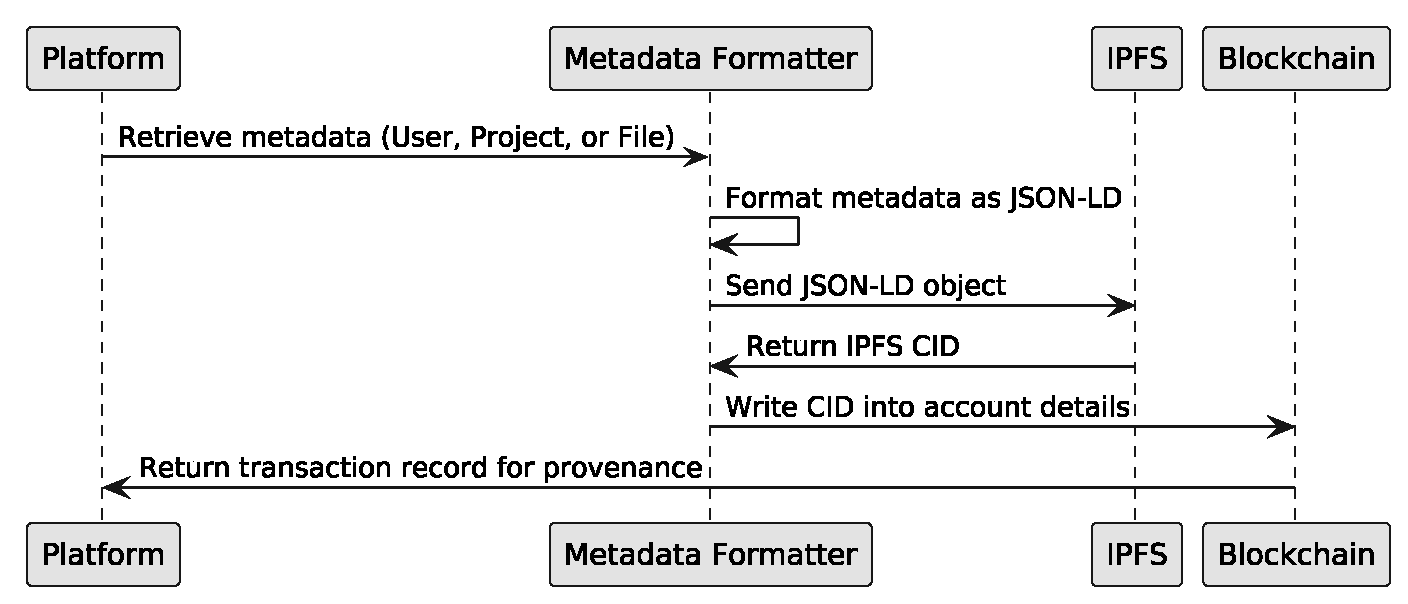
\includegraphics[scale=0.5]{fig/metadata_workflow_sequence.eps}
    \caption{Metadata workflow}
    \label{fig:metadata_workflow}
\end{figure}

\subsection{Blockchain Representation}

In the d-OSP, metadata for users, projects, and files are stored on the blockchain. This ensures the integrity and provenance of the metadata while leveraging decentralized technologies. The following subsections describe the structure of blockchain representations for both user and project data, as well as the files associated with these projects.

\subsection{User Account}

The representation of a user's account on the blockchain contains the standard Iroha v1 attributes for the account entity, such as the unique account identifier, domain information, and quorum for consensus. Additionally, the \texttt{json\_data} attribute references both the project to which the user is linked and the user's metadata CID (Content Identifier) stored on IPFS. This blockchain-based approach ensures that the user’s information remains immutable and traceable, which is critical for maintaining the integrity of research data.

Figures~\ref{fig:user_blockchain_representation} presents the JSON structure for account details for a user in the Iroha v1 blockchain.


\begin{listing}
    \begin{minted}[linenos=false,
               xleftmargin=21pt,
               tabsize=4,
               breaklines=true,
               breakanywhere=true]{json}
        {
        "account_id": "zealous_ptolemy@test",
        "domain_id": "test",
        "quorum": 1,
        "json_data": {
            "admin@test": {
                "linked_project": "02226@test",
                "account_metadata_cid": "QmT31fzDBNYAz1jAoAa7gQqSP7mDquv3fR8z1xLfxeHR5o"
            }
        }
    }
  
\end{minted}
    \caption{Blockchain Representation of User Account}
    \label{fig:user_blockchain_representation}
\end{listing}



\subsection{Project Account}

The project account representation similarly uses a blockchain-based structure to store project-related metadata. Each project is identified by a unique account ID, along with the project’s domain and quorum. The project metadata is linked to the user and includes important information about files associated with the project, including their CID references on IPFS. This ensures that the project data is linked to the user’s account and that all files and metadata related to the project are securely stored on the blockchain for provenance tracking.

The JSON structure describes the account details for a project in the Iroha v1 blockchain as shown in Figures~\ref{fig:project_blockchain_representation}.


\begin{listing}
    \begin{minted}[linenos=false,
               xleftmargin=21pt,
               tabsize=4,
               breaklines=true,
               breakanywhere=true]{json}
        {
        "account_id": "02226@test",
        "domain_id": "test",
        "quorum": 1,
        "json_data": {
            "admin@test": {
                "file_1": [
                    "QmTLZSqzPexwEdniZXLPN6fUfmEXX6MXS3b4QjKURgxc9y",
                    "Qmchg7At5whR1T4xP8TwTMd8ntQqJXbbSicJRtGGaW1Z2P"
                ],
                "linked_user": "zealous_ptolemy@test",
                "account_metadata_cid": "Qmay4cDaxUaZaHoJKqzN69XkiX8wMx17aG4VMmwmkLcL1a"
            }
        }
    }
  
\end{minted}
    \caption{Blockchain Representation of Project Account}
    \label{fig:project_blockchain_representation}
\end{listing}



\subsection*{File Representation}

Within the project account, each file associated with the project is represented by a CID pair. The first CID refers to the file stored on IPFS, while the second CID references the metadata associated with that file. This structure ensures that the file's content and its metadata are both stored and tracked independently, but are still linked to the blockchain for integrity and provenance.

\begin{itemize}
    \item The \textbf{first CID} (\texttt{QmTLZSqzPexwEdniZXLPN6fUfmEXX6MXS3b4QjKURgxc9y}) corresponds to the \textbf{file}.
    \item The \textbf{second CID} (\texttt{Qmchg7At5whR1T4xP8TwTMd8ntQqJXbbSicJRtGGaW1Z2P}) corresponds to the \textbf{metadata of the file}, ensuring that all relevant details are retrievable.
\end{itemize}

This structure allows for the efficient tracking and retrieval of research project data while maintaining provenance and integrity through blockchain storage.

%====================================================================
\section{Provenance}
\label{chp:proposed_model:sec:provenance}
%====================================================================

The provenance system takes a two-fold approach, with both methods being native features of their respective systems. The first approach leverages Iroha v1’s transaction logging capabilities, where each transaction is recorded with a hexadecimal hash and timestamp. This provides a reliable mechanism for tracking the evolution of account states over time. The hash acts as a snapshot, allowing for the retrieval of any past state of an account based on the corresponding transaction hash, as depicted in in Figure~\ref{fig:provenance}.

The second approach makes use of IPFS’s native feature of Content Identifiers (CIDs) to track metadata associated with accounts, projects, and files. Each piece of metadata is linked to a unique CID, which allows for decentralized storage and immutability. A mismatch of the CID indicates that the metadata or file has been modified, ensuring the integrity of the information over time.

Together, these two approaches, transaction logging through Iroha v1’s blockchain and metadata tracking through IPFS CIDs, provide a robust and transparent provenance system, ensuring both the transaction history and the integrity of metadata are verifiably recorded and traceable.


\begin{figure}[htbp]
    \centering
    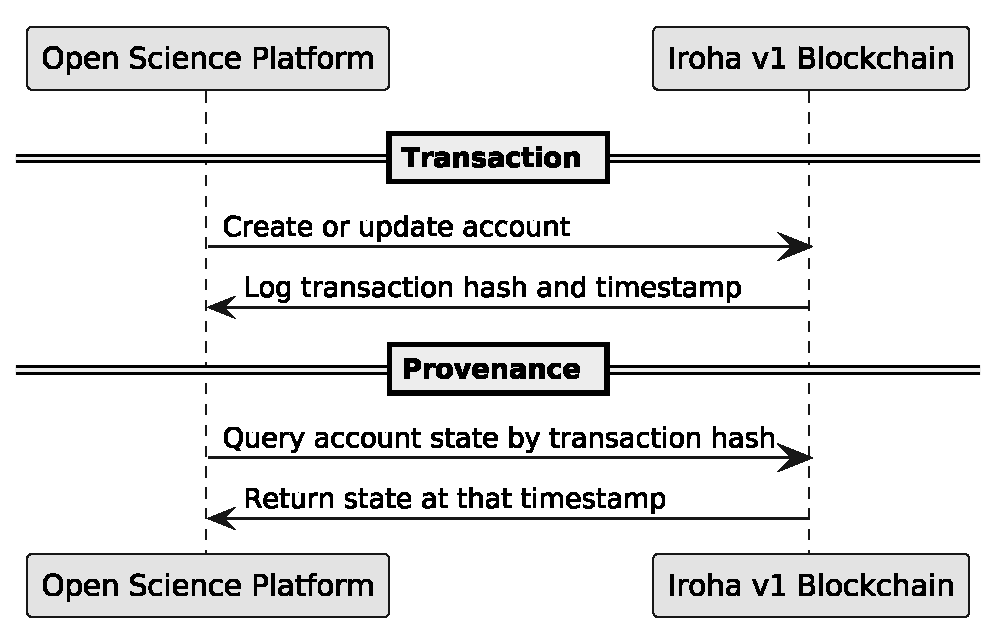
\includegraphics[scale=0.5]{fig/provenance_timeline.eps}
    \caption{Transaction logging and provenance query}
    \label{fig:provenance}
\end{figure}


%====================================================================
\section{Summary}
\label{chp:proposed_model:sec:summary}
%====================================================================

This chapter presents the d-OSP that provides a comprehensive and robust proposition for enhancing the reproducibility and transparency of scientific research. It leverages a modern technology stack comprising the Iroha v1 blockchain, InterPlanetary File System (IPFS), Jupyter Notebooks, Apache Tika, and Woosh. This stack ensures secure and efficient management of data and across the platform. The Iroha v1 blockchain, integrated with smart contracts and the Ethereum EVM compatible Hyperledger Burrow, guarantees the immutability and trustworthiness of all recorded actions, while IPFS enables decentralized storage of research data, ensuring scalability and resilience. Jupyter Notebooks serve as the primary front-end interface, providing an interactive environment for users to engage with research data. Apache Tika facilitates the extraction and processing of metadata from various document types, while Woosh powers advanced search and indexing functionalities, improving data discoverability and retrieval.

Platform operations are streamlined and well-defined. User enrollment and project registration are handled seamlessly through the Iroha v1 blockchain, where both users and projects are registered as accounts. This facilitates the management of roles, permissions, and interactions within the platform, ensuring efficient tracking. Research data management is integrated with the platform's metadata extraction system, allowing for the efficient storage and retrieval of research data that are consistently linked to their respective provenance, reinforcing the auditability of scientific outputs. Additionally, the search and validation functionalities provide users with tools to find, and explore research data.

The data model, represented through an Entity-Relationship (ER) model, underpins the platform's data structure, offering a flexible and comprehensive approach to managing users, projects, metadata, and research data. The role of metadata in the platform is crucial, as it is structured using well-established ontologies, including FOAF, Schema.org, and Dublin Core. These ontologies standardize the metadata representation, enabling interoperability and ensuring that all data is both machine-readable and discoverable. The integration of blockchain technology ensures that all metadata is transparently recorded, with the blockchain acting as a secure ledger for all metadata transactions, ensuring data integrity and facilitating trust in the platform. Provenance tracking is an essential aspect of the d-OSP, allowing for the tracing of data and results back to their origin, providing transparency, accountability, and enhancing the reproducibility of research.

%====================================================================
\chapter{Conclusions and Future Work}
\label{chp:conclusions}
%====================================================================

\begin{quotation}[British Philosopher (1902–1994)]{Karl Popper}
    Science is one of the very few human activities, \\
    perhaps the only one, \\
    where errors are systematically criticized and fairly often, in time, corrected.
\end{quotation}

\drop The ongoing reproducibility crisis has underscored the structural limitations of contemporary scientific practices, revealing systemic issues in transparency, accountability, and data accessibility. While Open Science has emerged as a response to these challenges, its implementation often remains constrained by centralized infrastructures that inadequately support verifiability and long-term data integrity. In contrast, the foundational tenets of decentralized technologies—immutability, distributed trust, provenance tracking, and censorship resistance—offer a compelling architectural framework to address these concerns. By integrating blockchain, smart contracts, and IPFS into a cohesive platform, it becomes possible to enforce transparent, tamper-evident records of research processes, enable automated compliance with reproducibility protocols, and ensure persistent access to underlying data and metadata.

This dissertation has demonstrated how such an integration can support a more trustworthy and verifiable scientific ecosystem, grounded in the principles of Open Science. The decentralized Open Science Platform (d-OSP) presented here exemplifies this potential, offering a technically grounded and ontologically structured response to reproducibility challenges. Although barriers remain—ranging from legal and infrastructural to usability and interoperability—the progress outlined in this work opens promising pathways forward. As this research draws to a close, the next phase will focus on advancing the platform's capabilities, ensuring broader adoption, and deepening its alignment with the evolving Open Science landscape. In doing so, this work aims to contribute meaningfully to reshaping the foundations of scientific practice in the digital age.

\newpage

This work has introduced a decentralized Open Science Platform (d-OSP) designed to address persistent challenges in scientific reproducibility and open research collaboration. By building on the integrated use of blockchain, IPFS, and smart contracts, the platform offers a cohesive technological foundation to support more transparent, verifiable, and collaborative research practices.

Reproducibility crises in science have often stemmed from a lack of traceable provenance, inaccessible data, opaque methodologies, and unreliable long-term availability of research artifacts. Centralized infrastructures tend to reinforce these issues by restricting control, limiting visibility, and introducing single points of failure. In contrast, decentralized technologies offer architectural characteristics that directly counter these systemic weaknesses.

Blockchain contributes immutability, auditability, and decentralized governance—ensuring that research records, once registered, are tamper-proof and independently verifiable. This integrity is fundamental to preserving the trustworthiness of experimental logs, provenance metadata, and contributions over time. Moreover, the use of smart contracts facilitates automated enforcement of verification processes and access control, providing reproducible workflows without dependence on centralized intermediaries.

IPFS complements this by enabling content-addressed and distributed storage, making research outputs—datasets, notebooks, protocols—available across a peer-to-peer network. This ensures persistent accessibility and efficient dissemination, both crucial for reproducibility and knowledge transfer.

Together, these technologies do not merely offer individual improvements, but form an integrated and synergistic approach to fulfilling the core propositions of open science: transparency, accessibility, verifiability, and collaboration. By enabling trustless interactions, distributed storage, and automated protocol enforcement, the d-OSP positions itself as a natural technical response to the reproducibility problem.

Looking ahead, the platform presents ample opportunities for continued development and refinement. Future work will focus on expanding artifact management capabilities, enhancing metadata extraction and search functionalities through deeper integration with knowledge graphs, and enabling support for complex, multi-source research data workflows. Research into domain-specific ontologies for scientific data will play a key role, alongside efforts to decentralize the deployment of the metadata parser and search engine. To foster a more engaged and collaborative research community, blockchain-based incentive mechanisms will be introduced to reward valuable contributions such as data sharing, result verification, and metadata enrichment. Further priorities include improving the overall user experience and implementing smart contract support for domain-specific logic, both of which are critical for the platform’s broader adoption and long-term impact.

In summary, the integration of decentralized technologies into scientific infrastructure is not an arbitrary technical upgrade, but a strategically aligned response to deeply rooted problems in reproducibility and openness. The d-OSP lays the groundwork for a future in which scientific knowledge is not only more accessible, but inherently more trustworthy and resilient.


\backmatter

% Appendices would be placed here	


\makeback{./Bibliography}


\end{document}
